\documentclass[12pt]{article}

\usepackage[utf8]{inputenc}
\usepackage[francais]{babel}

\usepackage{amsmath}
\everymath{\displaystyle}

\usepackage{caption}
\usepackage{subcaption}
\usepackage{float}

\usepackage{tikz}
\usetikzlibrary{calc}

\definecolor{densitylow}{RGB}{255,220,220}
\definecolor{densitymedium}{RGB}{255,130,130}
\definecolor{densityhigh}{RGB}{255,50,50}

\usepackage[natbib=true,sorting=none,style=numeric,url=false,doi=false,isbn=false]{biblatex}
%\addbibresource{references}
\bibliography{references}

\begin{document}

\begin{titlepage}

  Stage de recherche

  {\Large \textsc{Coévolution du réseau viaire et du bâti}}

  \begin{flushright}
    \textit{Auteur :}\\
    Merwan {\scshape Achibet}\\[0.5cm]
    \textit{Encadrants :}\\
    Stefan {\scshape Balev}\\
    Antoine {\scshape Dutot}\\
    Damien {\scshape Olivier}
  \end{flushright}

  \vfill

  \begin{center}
    ILLUSTRATION
  \end{center}

  \vfill

  \begin{center}
    
\includegraphics[width=.25\linewidth]{images/logo-univ-le-havre.png}
    \qquad\qquad\qquad
    
\includegraphics[width=.25\linewidth]{images/logo-litis.png}
  \end{center}

  \begin{center}
    {\small Mars - Juin 2012}
  \end{center}

\end{titlepage}

\begin{center}
  {\scshape\textbf Keywords}
\end{center}

{Urban system, city morphogenesis, Voronoi diagram, cellular automaton.}

\begin{center}
  {\scshape\textbf Extended abstract}
\end{center}

Gathering issues of human, economic, geographic and political nature,
the city truly is a complex system. The increasing growth in
population produces urban systems like the world has never seen
before, of increasing size, increasing heterogeneity and increasing
complexity. Studying the relationships between its internal elements
is fundamental to the understanding of its mechanics and to better
predict their developement. This work focuses on the relationship
between the pattern of human installations within the city --
characterized at the atomic level by a basic subdivision, the land lot
-- and its road network.

Systematic definitions of the city are many. Through the
anthropologist's eye it can be seen as a concentration of persons, the
economist will prefer to view it as a support for the exchange of
financial and physical assets and the urbanist as a functional entity
composed of flows and services. We choose to consider that the
evolution of a city is driven by its population, translated as a
measure of its density. This goes in hand with our focus, as land lots
are inhabited by the same people that uses the surrounding roads to go
from one place to another, and because urbanistic decisions are
motivated by a need to optimize the city, to streamline transport
means and to avoid high contrasts in the urban fabric.

A survey of the domain of urban simulations shows that available
scientific works can be classified into two categories. Methods have
been proposed for visual rendering purposes; they generate visually
satisfying cities without regarding realism as an obligation. These
are often based on empirical observations and their main idea is to
emulate the street patterns found in any urban system. Scientific
modeling, on the other hand, prefers to focus on the inner qualities
of a city, often by studying a subset of those, to analyze its current
state and extrapolate its future. We orient our research with the
latter in mind but the former represents a non-negligible source of
inspiration.

A reader browsing through the literature of the field will often
encounter cellular automata. The applicability and potential
complexity of these structures has been proven many times over and
they are fit for describing any kind of space-related
problem. Nevertheless, their rigorous formalism may sometimes restrain
realism and negatively impact the validity of the model. For example,
a cellular automaton topology is, by definition, perfectly
regular. Representing a city with a set of identical and aligned cells
seems like a coarse simplification. In the same way, we may question
the fact that each cell has an identical neighborhood structure, the
temporal synchronism and the state discretization. We take a drastic
step towards realism and embrace the spatial aspect of the city by
replacing the classic cellular automaton with a Voronoi diagram
following the same basic principle. Each of its cell represents a land
lot, and neighborhood relationships that are ruled by adjacency
determine its future state; the regularity constraint is thus
relaxed. Voronoi edges delineate the Voronoi space of land lots and,
as such, are ideal supports for roads.

The different elements represented in our model (\textit{i.e.} land
lots and roads) are declined in two flavors. \textit{Potential}
elements have an ethereal status; their spatial characteristics are
known but until they are effectively built, they have no direct effect
on the overall city and only represent an idea, a possible
outcome. \textit{Built} elements were potential elements that have
been constructed; they form the physical city. The gist of the model
is to add potential elements to the city and, only later, choose which
ones will be built and which ones will be forgotten. The road network
expands to accomodate the growth in density and to support anticipated
land lots. This process is divided into three separate mechanisms.

The cellular part of the model lets the inner variables of the city
vary based on the Voronoi tesselation and a set of simple rules. Here,
only population density is considered and, as a result, the
characteristic gradual patterns found in most towns are reproduced.

Whereas the previous part of the model is ensuring vertical growth,
the horizontal evolution of the city is handled by an extensible
method based on vector fields. Each piece of information that we want
to consider is represented by a vector field that will guide the
placement of new lots. For example, a field pointing away from high
density areas is used to ensure urban sprawl. Another field makes new
lots move towards the closest road such that they remain snapped to
the main transport axes. All vector fields are then summed up with
distinct factors. This general approach can model any kind of guidance
or constraint; in particular obstacle avoidance, so that the city
does not extends itself on forbidden areas like lakes, beaches or
protected forests.

The third and last mechanism chooses which of the potential elements
are to be permanently built. Potential roads are chosen with respect
to their contribution to the global network, by means of a network
flow evaluation. Potential land lots are chosen depending on their
position relative to the built roads and the date of their addition
into the potential domain.

RESULTATS/MESURES

\newpage

\tableofcontents

\newpage

REMERCIEMENTS

\newpage

\section{Introduction}

LES VILLES GRANDISSENT / STATISTIQUES

Le système complexe que forme la ville est donc soumis à une forte
croissance et un réel besoin de contrôler et de prévoir son évolution
se fait ressentir en conséquence de l'explosion démographique que
subissent les zones urbaines. C'est dans ce cadre de contrôle et de
prévision qu'il est nécéssaire d'étudier les mécanismes sous-jacents à
une ville pour pouvoir les reproduire sous forme de simulations et
étudier différents scénarios possibles.

On se concentre ici sur deux domaines majeurs du tissu urbain, le
viaire et le bâti, afin d'étudier leur relation de coévolution. Ces
deux aspects de la ville semblent aller de paire puisque le bâti
abrite les populations tandis que le viaire leur permet de se déplacer
d'un point à un autre. Il est ainsi naturel d'utiliser la densité de
population comme force de guidage de l'évolution de la ville.

EN DIRE PLUS

La première partie présente un état de l'art de la modélisation de
systèmes urbains et se concentre particulièrement sur les méthodes à
base d'automates cellulaires afin de metter en évidence leurs qualités
mais aussi les limitations qu'ils imposent. La structure de donneés et
les mécanismes régissant le modèle conçu dans le cadre de ce stage de
recherche sont ensuite présentés en seconde partie. Enfin, des mesures
diverses sont employées pour tester et valider ce travail dans la
troisième partie.

\section{\'Etat de l'art}

\subsection{Automates cellulaires et simulation urbaine}

La modélisation de systèmes complexes est longtemps uniquement passée
par l'usage de méthodes mathématiques; typiquement, des systèmes
d'équations différentielles. Ces techniques permettent de décrire des
lois d'évolution et d'observer, ainsi que de prédire par
extrapolation, le comportement de phénomènes du réel. Dans le cas de
modèles prenant en compte un vaste jeu de paramètres, cette approche
peut néanmoins se révéler délicate à employer. Plus intrinsèquement,
même si une telle modélisation est basée sur des observations ancrées
dans la réalité, il s'agit d'une représentation conceptuelle d'un
problème et aucune mimique des mécaniques sous-jacentes ne s'opère.

Historiquement, les prémices de l'informatique moderne et d'un tout
autre paradigme de modélisation sont à attribuer aux esprits du milieu
du vingtième siècle. Alan Turing introduit en 1936 la machine éponyme
qui, bien que purement théorique, possède un module de contrôle ainsi
qu'une mémoire et peut donc exécuter une infinité d'algorithmes. Cette
démarche se démarque de l'approche mathématique et semble plus
humaine; on ne résout pas un problème en utilisant des fonctions
associant une quantité à un résultat mais on agit véritablement sur
ses données. L'idée de base de Turing était d'ailleurs d'assimiler le
fonctionnement de sa machine au travail d'une personne remplissant les
cases d'un tableau infini.

Entraîné par cette mouvance procédurale et en réaction aux réseaux de
neurones de McCulloch et Pitts, John von Neumann et Stanislaw Ulam
joignent leurs travaux durant les années 40 pour concevoir l'automate
cellulaire : un système comprenant un ensemble d'automates à états
spatialement localisés (typiquement sous forme de grille) et
interconnectés en fonction de leur proximité. Les entrées de chaque
automate correspondent alors aux états des automates voisins et de
cette organisation se dégagent de fortes relations
d'interdépendance. Le jeu de la vie de Conway en est un exemple
classique. La simplicité de ses règles, mise en contraste avec la
variété des configurations engendrées, témoigne de la richesse des
automates cellulaires \cite{Gardner1970}.

Les automates cellulaires ont depuis été extensivement étudiés et sont
appliqués à l'étude de nombreux phénomènes biologiques, physiques et
sociaux \cite{Ganguly2003}. La motivation d'Ulam lors de leur
conception était d'ailleurs de modéliser la croissance de cristaux. On
peut aussi citer en exemple la simulation de la dynamique de fluides
\cite{Frisch1986} et de la croissance de tumeurs
\cite{Kansal2000}. Leur caractère spatial laisse supposer qu'ils sont
particulièrement adaptés aux applications géographiques et, dans le
cadre de notre problématique, urbaines. Ils ne fûrent paradoxalement
pas immédiatement exploités à cet effet et c'est seulement suite à un
article de Waldo Tobler, en 1975, que le rapprochement entre les
automates cellulaires et le domaine de la géographie apparaît
clairement \cite{Tobler1975}. Sont ensuite publiés des travaux majeurs
appliquant l'automate cellulaire à des problématiques géographiques
multi-échelles telles que l'évolution d'épidémies \cite{Fu2003} et la
ségrégation de population \cite{Schelling1969} (voir le modèle de
Schelling sur la figure \ref{fig:schelling}) et bien sûr la croissance
urbaine \cite{}. CITATIONS

\begin{figure}[H]
  \centering
  
\includegraphics[width=.5\linewidth]{images/schelling.png}
  \caption{Configuration produite par le modèle de Schelling. Chacune
    des deux couleurs représente une population différente. La
    conclusion de ces travaux est qu'un faible degré d'intolérance
    entre deux populations suffit à les séparer de manière évidente.}
  \label{fig:schelling}
\end{figure}

Une idée très exploitée dans ce domaine est d'associer un potentiel de
transition à chaque cellule et ce, vers tous les états qu'elles
peuvent adopter \cite{Benenson2004}. Dans les modèles déterministes,
la transition vers l'état à plus haut potentiel est appliquée tandis
que dans les modèles stochastiques, un tirage aléatoire biaisé est
préféré. Le potentiel d'une cellule à passer à un nouvel état est
déterminé en fonction de paramètres propres au modèle. Peuvent être
pris en compte l'élévation du terrain, la densité de population, la
proximité d'axes routiers, la proximité de centres urbains, l'âge des
parcelle, leur valeur; en fait, toute combinaison d'attributs relatifs
à un réseau urbain. Par exemple, dans une simulation représentant les
différents types d'usage, le passage d'une cellule à l'état
\textit{résidentiel} pourrait dépendre de la proximité des commerces
et des routes et de l'éloignement des zones industrielles. Bien sûr,
un nombre élevé de paramètres à prendre en compte requiert un couplage
fin et l'impact de chaque variable peut être pondéré. Puisque les
variations individuelles de paramètres n'émergent pas de manière
transparente à la surface de la simulation, les modèles urbains basés
sur des automates cellulaires doivent être finement calibrés et leur
réalisme est un défi en soi. Pour contourner ce problème, Yeh et Li
prônent l'usage d'un réseau de neurones pour pondérer chaque paramètre
à partir de l'analyse de données cartographiques historiques
\cite{Yeh2002}.

Il est important de noter que la simplicité du formalisme enveloppant
un automate cellulaire strict s'oppose à la fidélité de la simulation,
notamment dans le cadre de modèles spécifiques
\cite{Torrens2000,Torrens2001}. Dans ce cas, une prise de liberté
quant aux formalisme originel est autorisée, voire nécessaire, pour
obtenir des résultats satisfaisants \cite{White1998}.

La première limite que le formalisme cellulaire de base impose est la
discrétisation des états que chaque cellule peut adopter. Même si
cette caractéristique fait partie intégrante des particularités qui
confèrent aux automates cellulaires leur simplicité d'usage et
d'analyse, la description de quantités pouvant arborer un éventail
infini de valeurs est alors impossible. Plus concrètement, il est aisé
de catégoriser les cellules d'un espace selon le fait, par exemple,
qu'elles contiennent des installations humaines ou non (état booléen)
\cite{Benguigui2004,Cornu2008} ou de façon plus sophistiquée, en
fonction de leur type d'usage (\textit{résidentiel},
\textit{commercial}, \textit{industriel} \cite{Lechner} et plus
\cite{Dubos-Paillard2003}). Représenter des quantités réelles et des
variations continues l'est moins. Pour symboliser plus finement la
densité au c\oe ur d'un ensemble urbain, Semboloni utilise par exemple
un automate cellulaire de dimension trois dans lequel plus une pile de
cellules actives est haute et plus la zone représentée est peuplée
\cite{Semboloni2000}. Plus généralement, il est accepté de représenter
l'état d'une cellule par un vecteur contenant des valeurs réelles; des
règles de transitions adaptées et mesurées sont alors à mettre en
place.

L'homogénéité d'un automate cellulaire fait partie intégrante de sa
définition originelle : en mettant de côté l'état qu'elles adoptent,
toutes les cellules sont identiques en forme et en structure de
voisinage. Dans le cadre de notre problématique, cette approche est
limitante car, dans une ville, les parcelles ne sont
qu'occasionnellement identiques et alignées. Similairement, la notion
de voisinage est clairement à redéfinir. Classiquement, les voisinages
de von Neumann et de Moore sont utilisés mais la relation par
contiguité qu'ils décrivent ne convient pas à la représentation des
liens de dépendance à plus grande échelle se développant dans un
système urbain. Le positionnement d'un bâtiment résidentiel dans une
ville se base évidemment sur le voisinage direct des zones envisagées
(on préfère construire une maison dans un quartier résidentiel) mais
il faut aussi prendre en compte les alentours plus distants (la
centrale thermique se trouvant à 500 mètres du site peut poser
problème). Une solution possible est d'étendre les aires des
voisinages de von Neumann et de Moore tout en conservant leur forme
caractéristique. La symétrie évidente se dégageant de telles
simplifications va à l'encontre des relations prenant place au sein
d'une ville. O'Sullivan a choisi de relaxer cette contrainte de
partionnement spatial régulier pour faire un pas dans la direction du
réalisme en proposant l'automate cellulaire graphe
\cite{O'Sullivan2000,O'Sullivan2001}. Conventionnellement, une cellule
d'automate correspond à un sous-espace urbain ou bien une parcelle
cadastrale mais dans chacun de ces cas le modèle se base évidemment
sur une simplification grossière de l'espace étudié. Il décide donc de
donner à chaque cellule les mêmes qualités topologiques que les
parcelles qu'elles représentent : même formes, même dimensions, mêmes
coordonnées. Une variété de relations de voisinage sont alors
envisageables (par voisinage au sens urbain, par distance dans un
rayon d'influence, par critère de visibilité). L'éloignement du
formalisme cellulaire est drastique car la structure perd de son
homogénéité puisque chaque cellule est différente et chaque voisinage
est unique. Il faut aussi noter que la couverture de l'espace n'est
plus complète car des vides entre les cellules apparaissent. Chacune
des ces concessions est mise au service du réalisme de la
simulation. Un exemple de sous-espace urbain représenté par ce modèle
est visible sur la figure \ref{fig:sullivan}.

\begin{figure}[H]
  \centering
  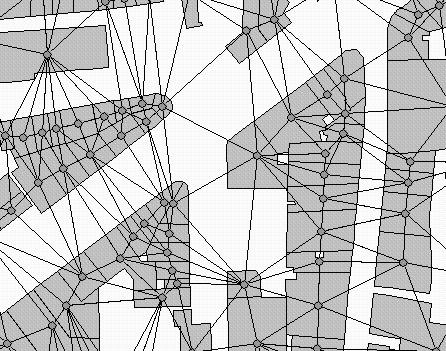
\includegraphics[width=.7\linewidth]{images/gca.png}
  \caption{Hoxton, un quartier de Londres, modélisé par l'automate
    cellulaire graphe de David O'Sullivan \cite{O'Sullivan2000}.}
  \label{fig:sullivan}
\end{figure}

Une prise de liberté quant à l'aspect temporel est aussi
envisageable. Un automate cellulaire strict est synchrone,
\textit{i.e.} les changements d'état de toutes les cellules
s'effectuent simultanément. Si le choix était fait de mettre à jour
chaque état de façon asynchrone, le comportement de l'automate en
serait lourdement modifié. Par exemple, les qualités auto-réplicatives
de certaines entités du jeu de la vie ne seraient pas garanties. Il
est pourtant légitime de se questionner sur la validité d'un tel choix
dans une simulation urbaine; premièrement parce qu'une ville est un
système complexe et désordonné, ensuite parce les processus qui s'y
déroulent sont réglés sur différentes échelles temporelles.

Bien que les automates cellulaires soient couramment utilisés pour
simuler le trafic routier (dans leur version 1D ou 2D
\cite{Queloz1996}), ils s'accordent peu avec la construction même d'un
réseau viaire. Dans les simulations cellulaires urbaines, le
positionnement des routes a un impact sur le développement des
cellules puisque le viaire \textit{attire} le bâti mais le réseau est
souvent fourni en entrée et reste statique. Nous sommes amener à nous
interroger sur la capacité des automates cellulaires à modéliser le
développement routier car la cellule n'est pas une représentation
adéquate d'une structure linéaire dont l'échelle est plus large que
celle de la parcelle.

\subsection{Approches alternatives}

Les automates cellulaires ne sont pas l'unique moyen de modéliser la
croissance urbaine. Plusieurs simulations existantes sont des systèmes
multi-agent \cite{Lechner2003,Lechner2004}. Dans ces cas, un agent est
assimilé à un promoteur immobilier et peut acheter des terres, les
vendre, les développer ou changer leur type. Les actions qu'il
entreprend sont évaluées en fonction de l'impact sur la ville
(changement de la valeur immobilière, avis de la population) et des
réglementations locales afin d'éviter toute configuration illégale.
Pour la construction du réseau routier, une solution est de mettre en
place, en plus des agents promoteurs, deux types d'agents
traceurs. Les \textit{extenders} parcourent toute la surface du
terrain à la recherche de bâtiments isolés et éloignés puis tracent
une nouvelle route jusqu'au réseau urbain. Les \textit{connectors} se
déplacent uniquement sur le réseau viaire et y raccordent les
bâtiments non connectés se trouvant dans leur rayon de détection
\cite{Lechner2003}. Cette approche introduit un défaut conceptuel : le
réseau viaire est construit à partir du bâti et non l'inverse. Ainsi,
des bâtiments peuvent rester isolés pendant plusieurs itérations de la
simulation et, même si le résultat final apparaît comme satisfaisant,
arrêter la simulation en cours de l'évolution du système produit une
configuration erronée. Autrement dit, l'évolution n'est pas
historiquement cohérente et seule la ville finale est correcte.

Un autre modèle gérant à la fois l'évolution du réseau viaire et du
bâti est présenté par Weber \cite{Weber2009}. Le principe est le
suivant : à chaque agrandissement du réseau urbain, on crée plusieurs
routes éphémères en suivant des règles géométriques précises
(allongement des voies existantes, limitation du degré des carrefours
à 4, l'angle entre chaque rue tend vers 90 degrés). Parmi les $n$
routes générées, une seule sera construite. Pour la choisir, le trafic
sur ces nouvelles routes est simulé par des agents piétons et
véhicules et l'on identifie celle qui sera la plus globalement
bénéfique au réseau.

Barthelemy et Flammini \cite{Barthelemy2009} proposent aussi un modèle
dans lequel le viaire et le bâti évoluent simultanément. Le bâti,
représenté par une mesure de densité sur des points disposés
régulièrement dans l'espace, croît linéairement en fonction du
temps. Le réseau routier s'agrandit en suivant des règles empiriques
\cite{Barthelemy2008} associées à un critère de proximité tel qu'une
voie passant entre deux points de densité s'en trouvent à distances
égales. Il est intéressant de noter que, sans le mentionner, les
auteurs construisent ainsi un diagramme de Voronoï partiel comme celui
qui est à la base de notre modèle.

D'autres solutions s'éloignant des systèmes complexes et penchant du
côté de la génération procédurale de contenu existent
\cite{Kelly2006}. Souvent, le domaine d'application de telles méthodes
est l'infographie, le cinéma et le jeu vidéo. L'objectif est alors de
construire de manière automatique une ville visuellement réaliste sans
se soucier de son caractère fonctionnel. Usuellement, l'organisation
parcellaire dépend entièrement du réseau routier car la première étape
est souvent de générer un réseau viaire complet puis de placer le bâti
en subdivisant récursivement les niches vides formées par les
voies. Dans Citygen \cite{Kelly2006b}, un point $p$ de l'espace est
aléatoirement choisi puis on calcule un ensemble de plusieurs routes
raccordant $p$ au réseau routier existant en faisant varier leur
déviation angulaire et un paramètre de bruit; la route finale est
celle pour laquelle la variation d'altitude est la plus
faible. CityEngine \cite{Parish2001} utilise un L-System dont les
règles permettent de reproduire les différents motifs quadrillés,
radiaux et organiques que l'on retrouve dans une ville. La nature
récursive des L-Systems permet à ces motifs de se combiner et
d'apparaître à différents niveaux de profondeur (voir figure
\ref{fig:cityengine}). Dans une autre simulation, le tracé des routes
suit les \textit{hyperstreamlines} \cite{Chen2008} formées par un
champ de vecteurs. Ce champ est calculé par combinaison de plusieurs
autres champs de vecteurs, chacun représentant des contraintes
directionnelles particulières telles que les zones interdites,
l'altitude et le directives données par l'utilisateur. Ces techniques
sont intrinsèquement géométriques, et comme précisé plus haut, le
résultat est purement visuel; elles représentent néanmoins une source
d'inspiration à ne pas négliger.

\begin{figure}[H]
  \centering
  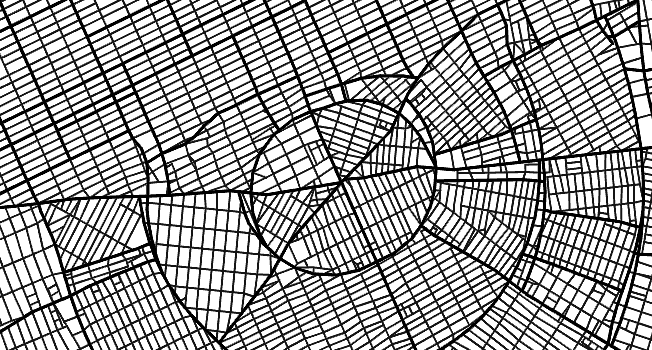
\includegraphics[width=.8\linewidth]{images/cityengine.png}
  \caption{CityEngine mélange des motifs urbains extraits de cartes de
    Paris et de New York \cite{Parish2001}.}
  \label{fig:cityengine}
\end{figure}

\section{Le modèle}

\subsection{Structure}

Les automates cellulaires sont des structures versatiles et puissantes
dont le formalisme originel impose néanmoins quelques limitations;
l'une des principales étant, à nos yeux, un maillage régulier et
statique. Pour répondre à notre problématique, il est nécessaire
d'employer une structure respectant les critères suivants :

\begin{enumerate}
\item{Elle doit partitionner l'espace, possiblement de façon
  irrégulière;}
\item{Des relations de voisinages pourront être déduites de sa
  topologie;}
\item{Elle doit pouvoir représenter à la fois la parcellisation du
  territoire et le réseau routier.}
\end{enumerate}

Le diagramme de Voronoï est un candidat idéal. Sa constitution est
intrinsèquement spatiale puisqu'il s'agit d'un partionnement axé
autour de points spéciaux, les générateurs, chacun possédant une
cellule contenant tous les points plus proches de ce générateur que de
tout autre. Autrement dit, la distance séparant un point $p$ placé
dans une cellule de Voronoï et le générateur de cette même cellule est
inférieure à la distance séparant $p$ de tous les autres générateurs
\cite{Edwards1993}. La figure \ref{fig:voronoi} fournit un exemple de
diagramme de Voronoï. On remarque visuellement quelques propriétés
notables; notamment le fait que deux générateurs voisins sont
équidistants de l'arête les séparant et que le segment les reliant y
est perpendiculaire.

\begin{figure}[!ht]
  \centering
  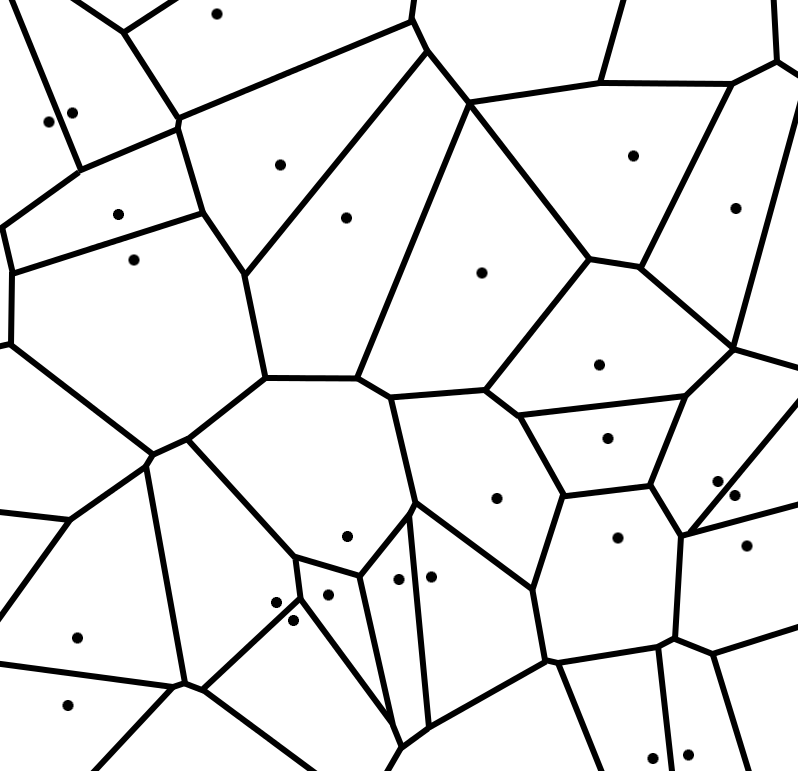
\includegraphics[width=0.7\linewidth]{images/voronoi.png}
  \caption{Un diagramme de Voronoï. Chaque point noir est un générateur.}
  \label{fig:voronoi}
\end{figure}

Les diagrammes de Voronoï trouvent de nombreuses applications en
science. En robotique, les obstacles présents dans un environnement
peuvent être assimilés à des générateurs et un robot cherchant à
maximiser leur évitement préférera longer les frontières des cellules
(les arêtes de Voronoï) \cite{Garrido2006}. En sociologie
géographique, ils permettent d'opposer les zones d'influence de
différents éléments urbains et répondent à des questions telles que :
quel magasin un piéton sera-t-il plus susceptible de visiter selon la
zone dans laquelle il se trouve ? Leur utilisation pour l'étude de
l'épidémie de choléra londonienne en 1854 à permis de vérifier le lien
entre fontaines publiques infectées (les générateurs) et zones
souffrant d'un fort taux de mortalité (les cellules)
\cite{Thomas2010}.

Comme son homonymie le laisse présager, la cellule de Voronoï remplace
dans notre modèle la cellule de l'automate cellulaire. Une grille
régulière, comme celles présentes dans les automates cellulaires
classiques, correspond d'ailleurs à un diagramme de Voronoï dans
lequel les générateurs sont régulièrement disposés. Une tesselation de
Voronoï peut être considérée comme une généralisation de la structure
grillagée; notre première contrainte est donc satisfaite.

À l'échelle de ce modèle, chaque cellule représente une parcelle
cadastrale et on utilise comme générateur le centre de l'empreinte de
la parcelle. Le diagramme permet d'identifier les parcelles voisines
comme étant celles partageant une arête de Voronoï. Un graphe de
voisinage est ainsi construit et adopte la forme duale du diagramme de
Voronoï : la triangulation de Delaunay (voir figure
\ref{fig:delaunay}). Les structures de voisinage de chaque cellule
sont déterminées à partir de la topologie du diagramme et la seconde
contrainte est satisfaite.

\begin{figure}[!ht]
  \centering
  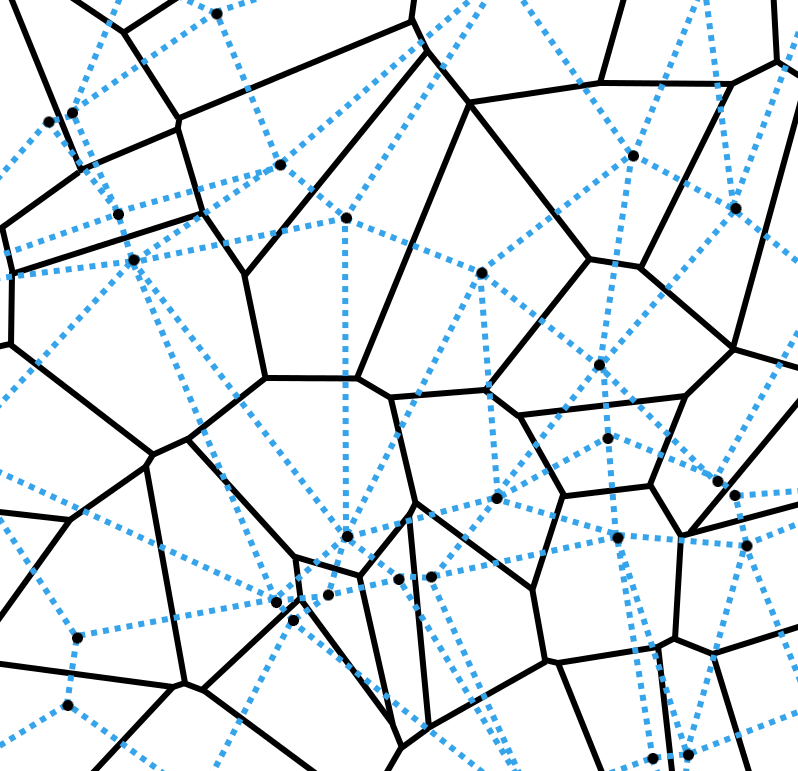
\includegraphics[width=.7\linewidth]{images/delaunay.png}
  \caption{le réseau de voisinage du diagramme de Voronoï (en noir)
    correspond à sa forme duale, la triangulation de Delaunay (en
    bleu).}
  \label{fig:delaunay}
\end{figure}

Le diagramme de Voronoï permet de décrire un canevas urbain de base
dans lequel l'espace d'influence de chaque parcelle est décrit mais la
composante routière reste encore absente du modèle. Chaque arête de
Voronoï indique un espace entre deux parcelles et est donc susceptible
d'accueillir une route. Bien sûr, dans une véritable ville, chaque
parcelle n'est pas encerclée de voies; l'un des objectifs du modèle
est de déterminer quelles arêtes accueilleront des routes et quelles
arêtes resteront vides. Cette structure suffit donc à représenter à la
fois les éléments du viaire et du bâti. Notre dernière contrainte est
comblée.

En pratique, dans notre modèle un système urbain est représenté par
deux graphes : le graphe viaire et la graphe de voisinage du bâti. Le
graphe du bâti a pour n\oe ud les centres des parcelles et ses arêtes
symbolisent les relations de voisinage. Le graphe viaire a des arêtes
représentant les routes et des n\oe uds représentant les
carrefours. Les structures de ces graphes sont basées sur la topologie
du diagramme de Voronoï puisqu'il s'agit pour le graphe viaire de
l'ensemble des arêtes et sommets de Voronoï et pour le graphe du bâti,
de sa triangulation de Delaunay.

Il est essentiel de dissocier le polygone convexe qu'est la cellule de
Voronoï et la véritable empreinte cadastrale de la parcelle qu'elle
répresente. Une cellule représente l'influence d'une parcelle dans
l'espace urbain et possède comme seul point commun avec l'empreinte
son centre puisqu'il s'agit du générateur de la
cellule. Similairement, une arête peut indiquer qu'une voie passe
entre deux parcelles sans pour autant fournir ses coordonnées ou sa
courbure. Si l'on souhaite, dans un but infographique, générer une
image de notre ville à partir de ce modèle, un travail
d'interprétation est nécessaire et n'a pas été traîté à l'occasion de
ce projet. Un exemple est visible sur la figure \ref{fig:interp}.

\begin{figure}[H]
  \centering
  \subcaptionbox{}[0.9\linewidth][c]{
    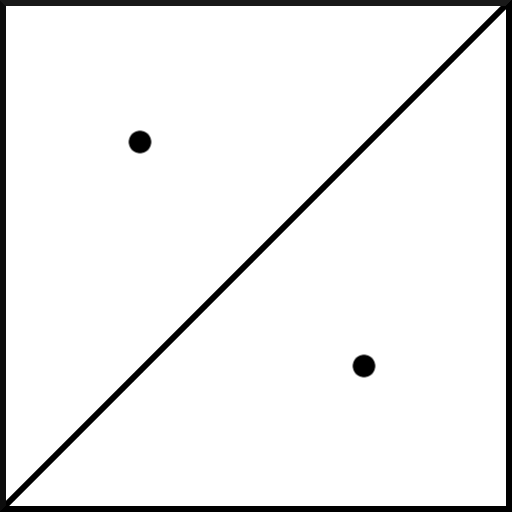
\includegraphics[width=.3\linewidth]{images/voronoi-interp0.png}
  }

  \subcaptionbox{}[.3\linewidth][c]{
    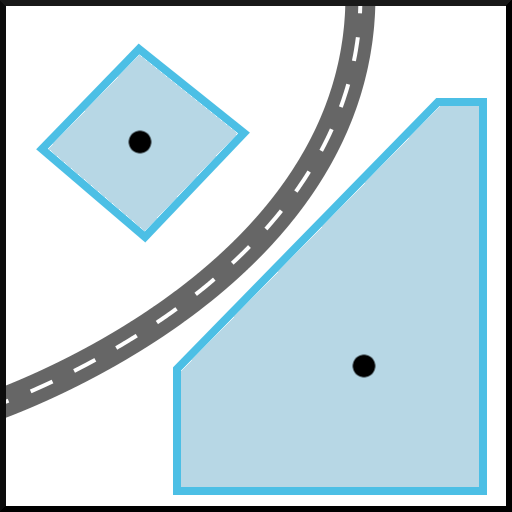
\includegraphics[width=.3\linewidth]{images/voronoi-interp1.png}
  }
  \subcaptionbox{}[.3\linewidth][c]{
    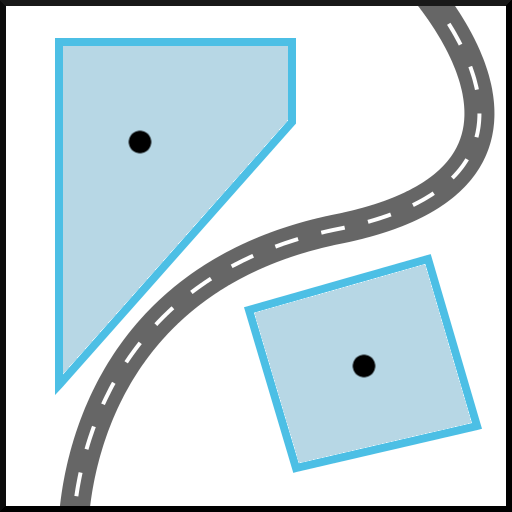
\includegraphics[width=.3\linewidth]{images/voronoi-interp2.png}
  }
  \subcaptionbox{}[.3\linewidth][c]{
    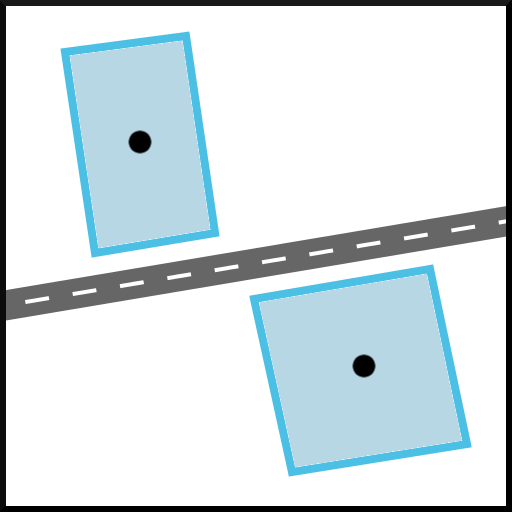
\includegraphics[width=.3\linewidth]{images/voronoi-interp3.png}
  }
  \caption{Un diagramme de Voronoï trivial et trois interprétations possibles.}
  \label{fig:interp}
\end{figure}

\subsection{Potentialité}

Via le terme \textit{potentialité}, on souhaite exprimer l'opposition
entre deux types d'éléments : les \textit{potentiels} et les
\textit{construits}.

Un élément \textit{construit} est une parcelle ou une voie dont
l'existence physique est avérée et qui affecte ses
alentours. L'ensemble des éléments construits forme la ville.

Un élément \textit{potentiel} peut être assimilé à une idée germant
dans l'esprit de l'urbaniste; à une possibilité envisagée et
représentée de manière intangible mais néanmoins précise. Les
parcelles potentielles, particulièrement, n'ont pas d'effet sur le
bâti construit. Par contre, elles attirent la construction des routes.

\begin{figure}[H]
  \centering \subcaptionbox{}[.45\linewidth][c]{
    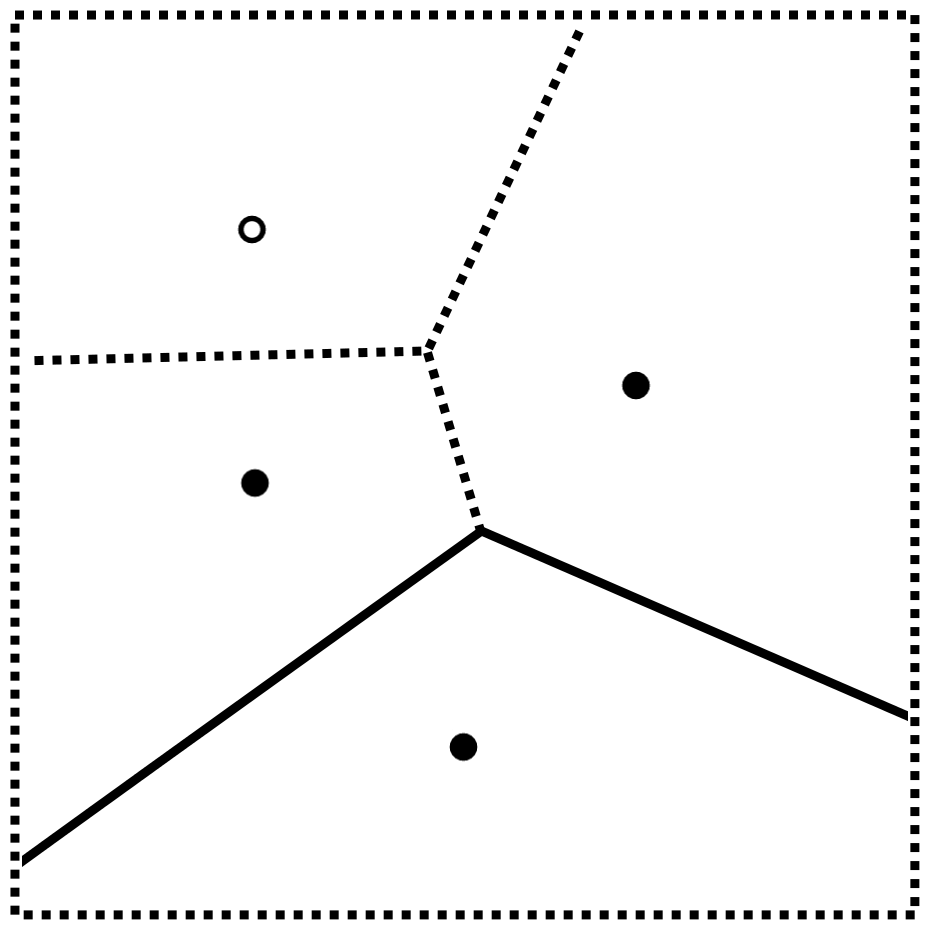
\includegraphics[width=.45\linewidth]{images/potential-voronoi.png}
  }
  \subcaptionbox{}[.45\linewidth][c]{
    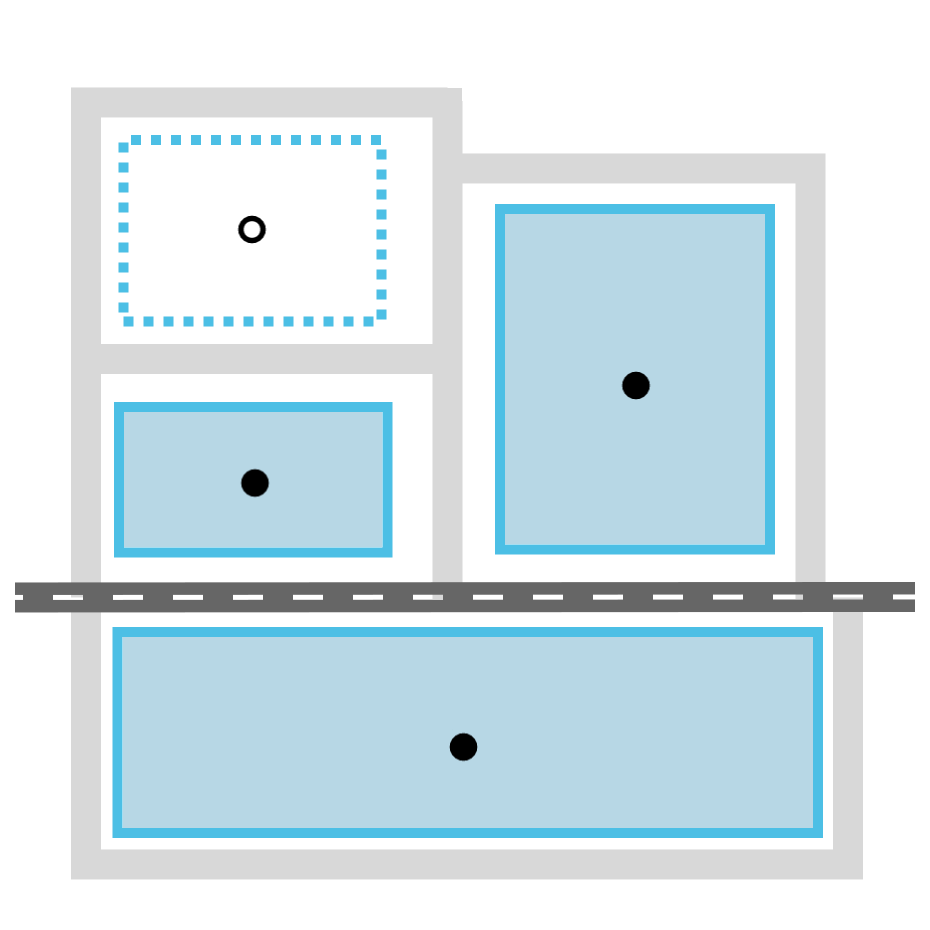
\includegraphics[width=.45\linewidth]{images/potential-interp.png}
  }
  \caption{}
  \label{fig:potentialite}
\end{figure}

Cette dualité et cette unidirectionalité sont justifiées par un désir
de fournir un modèle historiquement cohérent. On ne se contente pas de
générer itérativement un système urbain complet et de considérer la
configuration finale comme l'unique résultat. Chaque itération fournit
un résultat en soi et assembler chaque instantané de la ville doit
décrire sa croisance naturelle.

Si l'on souhaite reproduire le cycle d'urbanisation prenant place dans
une vraie ville, la question de l'ordonnancement des étapes se
pose. L'implantation de nouveaux bâtiments est lourdement dépendante
du réseau routier existant puisqu'on ne construit pas
d'infrastructures isolées des axes de transport. \`A l'inverse, le
développement du réseau viaire est dépendant du bâti puisque la
fonction des routes est avant tout de le desservir. En partant de ce
constat, nous sommes face à un problème dans lequel chaque domaine
traîté est dépendant de l'autre. Donc, faut-il construire la bâti puis
le relier au réseau viaire ? Faut-il installer les routes puis les
peupler par du bâti ?  L'\oe uf ou la poule ? La figure
\ref{fig:bati-viaire} résume cette situation d'interdépendance.

\begin{figure}[H]
  \centering
  \begin{tikzpicture}

  \node[draw,rectangle] (b) at (-1,0) {Bâti};
  \node[draw,rectangle] (v) at (+1,0) {Viaire};

  \draw (b.north) edge[->,out=90,in=90] (v.north);
  \draw (v.south) edge[->,out=-90,in=-90] (b.south);

\end{tikzpicture}

  \caption{}
  \label{fig:bati-viaire}
\end{figure}

Lors de la croissance des villes, le cyle d'urbanisation se déroulant
est le suivant :

\begin{enumerate}
\item{Une nouvelle installation est prévue en bordure de la ville,
  dans une zone posiblement isolée du réseau routier;}
\item{Une route est construite pour permettre l'installation de la
  nouvelle parcelle;}
\item{Une fois la route contruite, la parcelle peut être à son tour construite;}
\item{D'autres parcelles vont se construire sur la nouvelle route.}
\end{enumerate}

\begin{figure}[H]
  \centering \subcaptionbox{}[.24\linewidth][c]{
    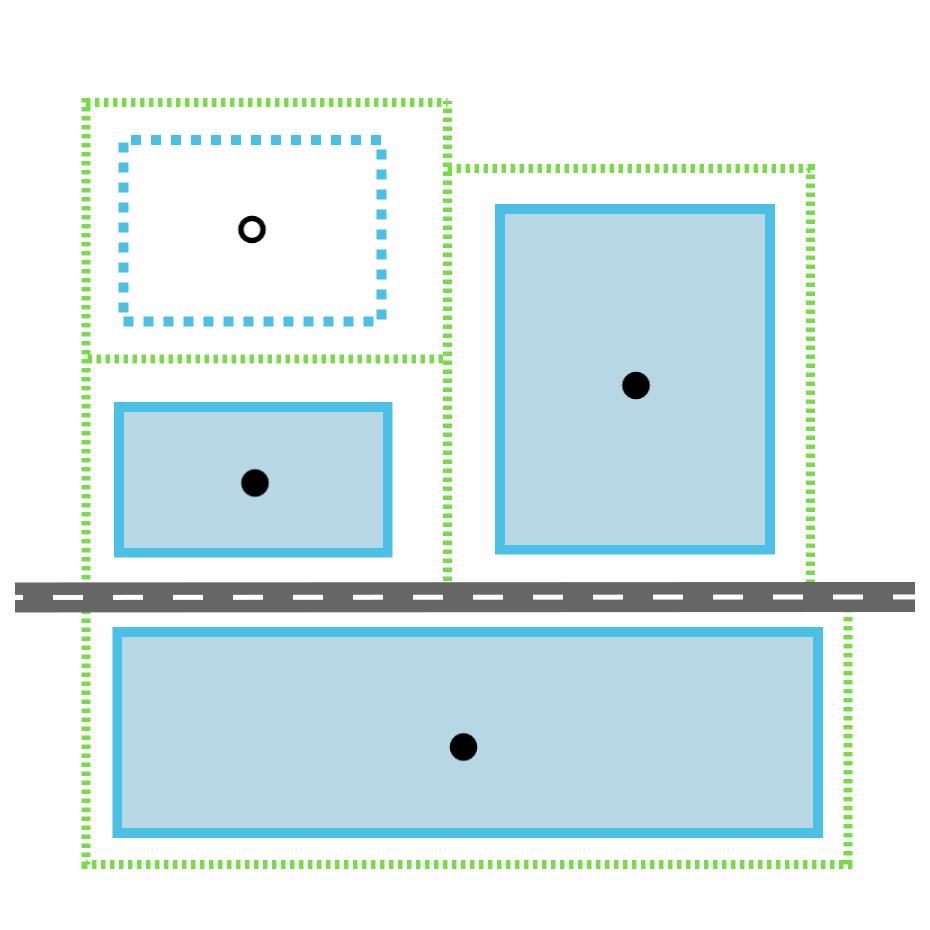
\includegraphics[width=.24\linewidth]{images/order_good_0.png}
  }
  \subcaptionbox{}[.24\linewidth][c]{
    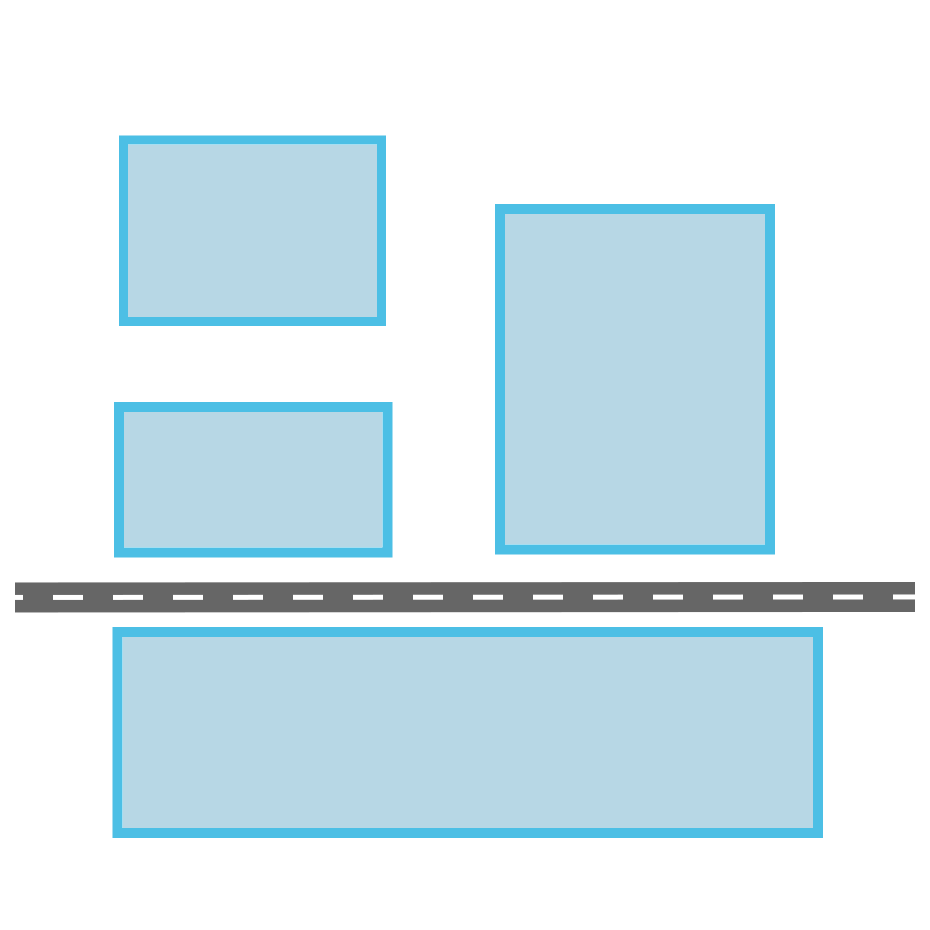
\includegraphics[width=.24\linewidth]{images/order_bad_1.png}
  }
  \subcaptionbox{}[.24\linewidth][c]{
    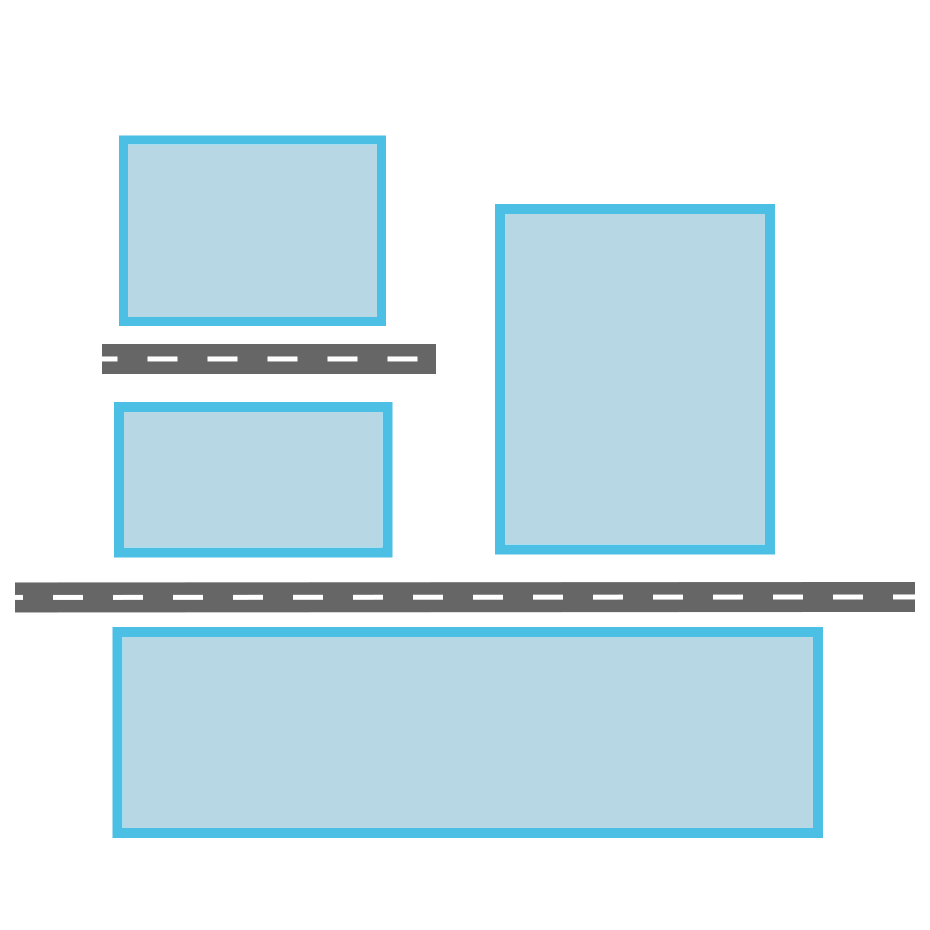
\includegraphics[width=.24\linewidth]{images/order_bad_2.png}
  }
  \subcaptionbox{}[.24\linewidth][c]{
    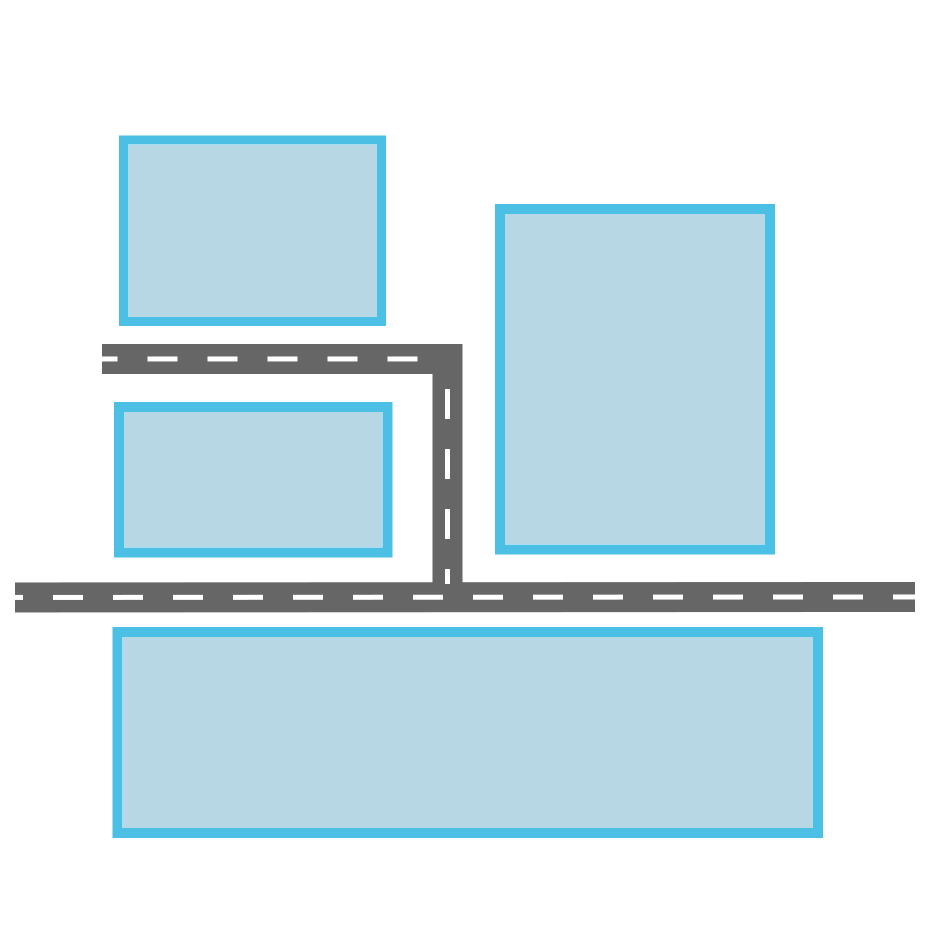
\includegraphics[width=.24\linewidth]{images/order_good_3.png}
  }
  \caption{}
  \label{fig:order-bad}
\end{figure}

\begin{figure}[H]
  \centering \subcaptionbox{}[.24\linewidth][c]{
    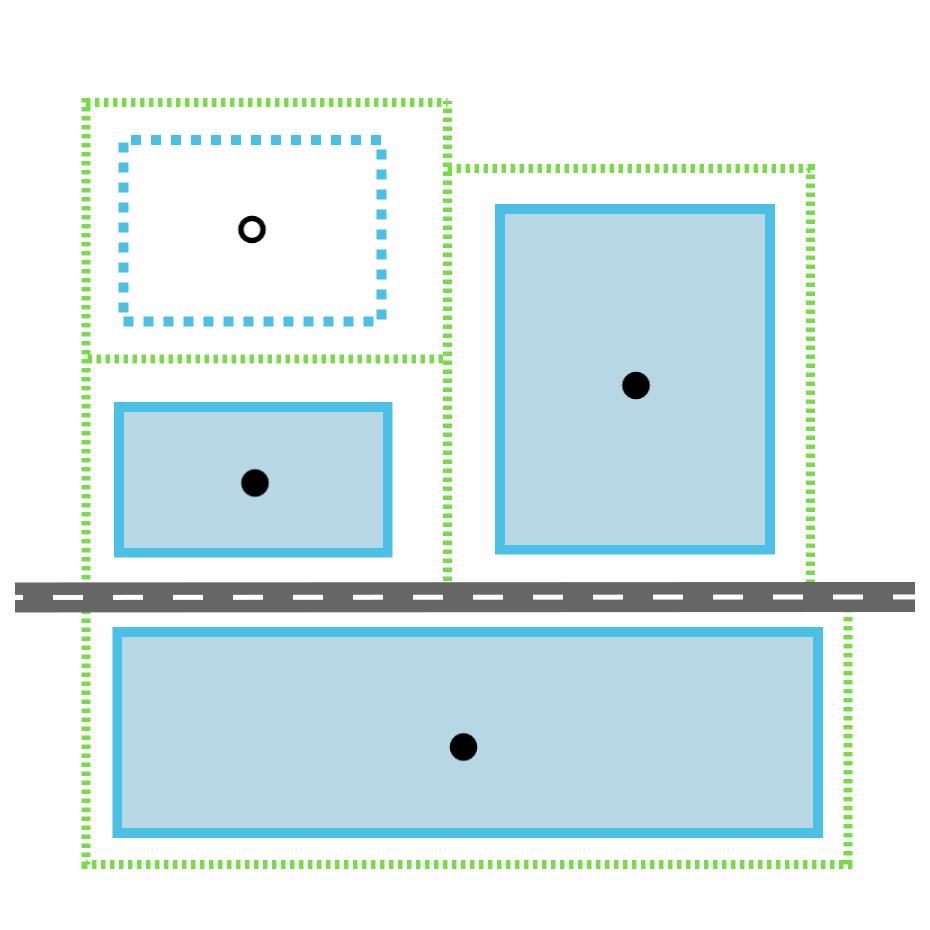
\includegraphics[width=.24\linewidth]{images/order_good_0.png}
  }
  \subcaptionbox{}[.24\linewidth][c]{
    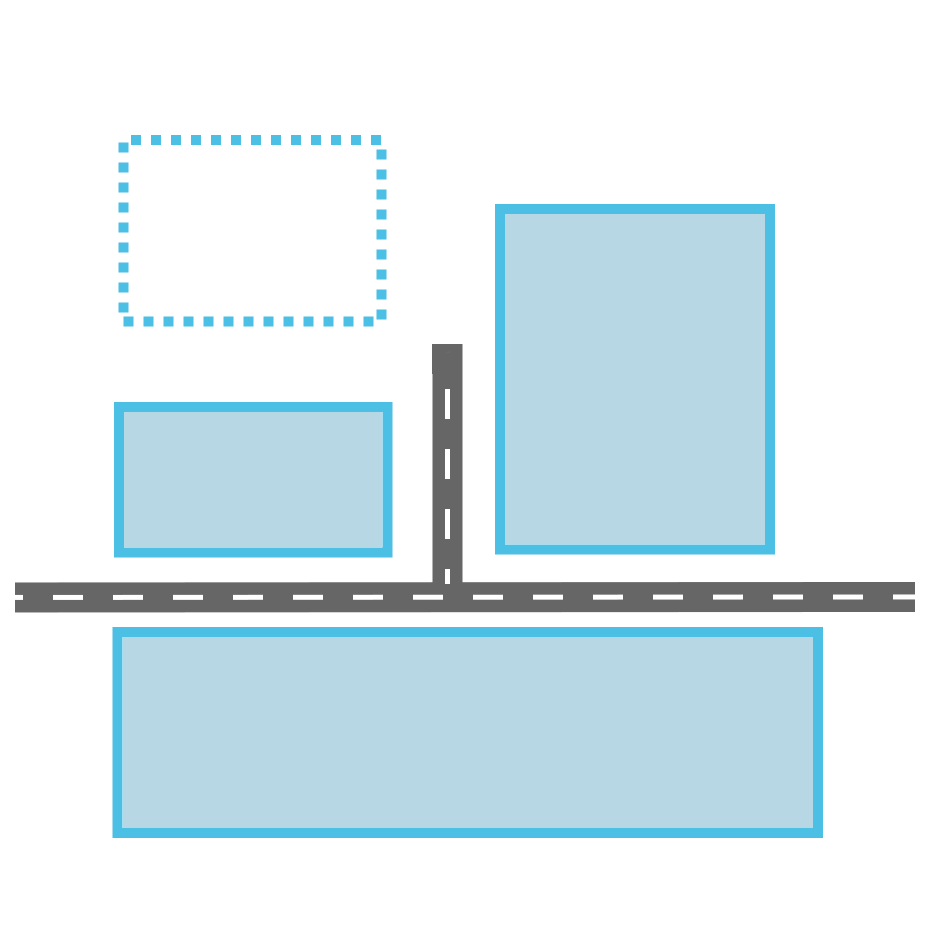
\includegraphics[width=.24\linewidth]{images/order_good_1.png}
  }
  \subcaptionbox{}[.24\linewidth][c]{
    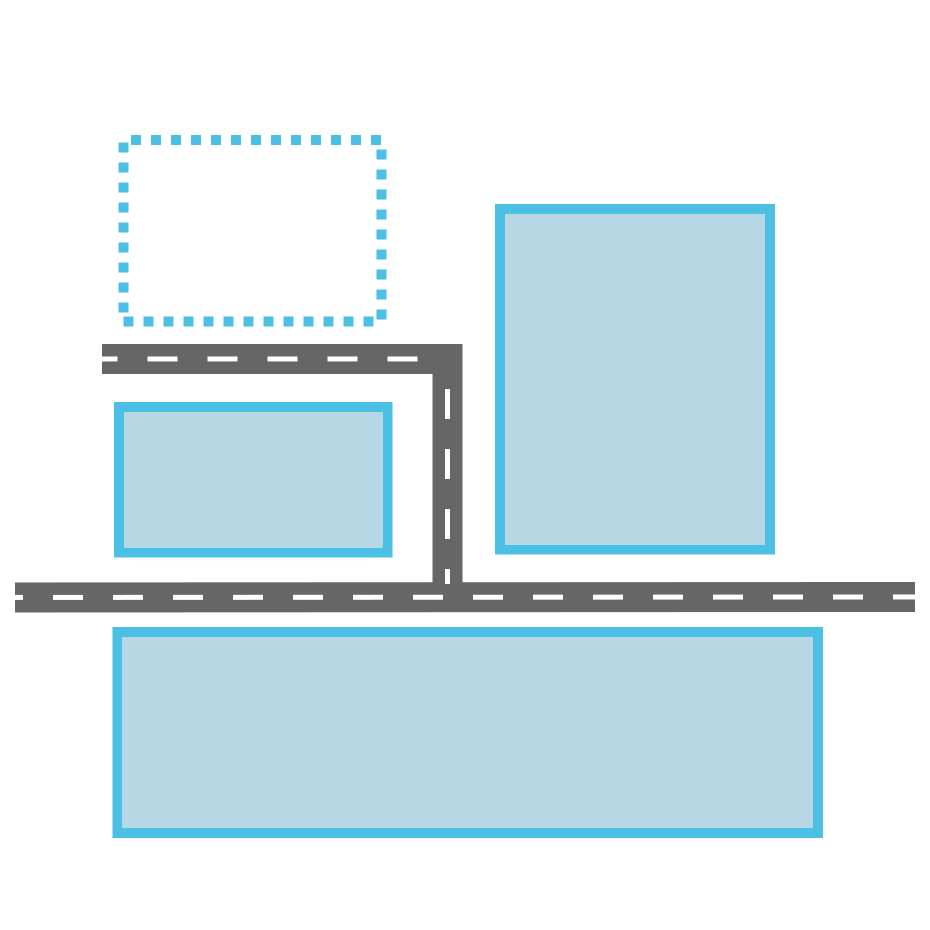
\includegraphics[width=.24\linewidth]{images/order_good_2.png}
  }
  \subcaptionbox{}[.24\linewidth][c]{
    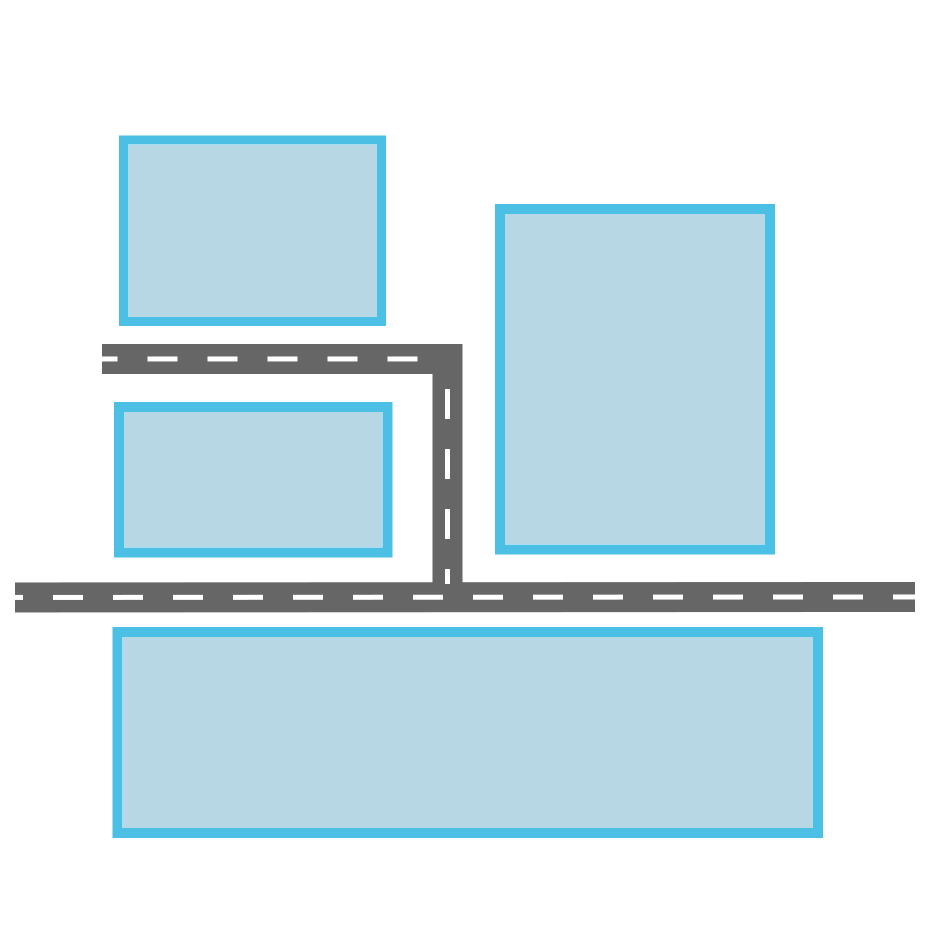
\includegraphics[width=.24\linewidth]{images/order_good_3.png}
  }
  \caption{}
  \label{fig:order-good}
\end{figure}

Dans notre modèle, ces quelques étapes se traduisent comme suit :

\begin{enumerate}
\item{Une parcelle potentielle est placée dans une zone vide;}
\item{On construit les routes potentielles menant à la parcelle
  potentielle;}
\item{Une fois la route contruite, la parcelle peut être à son tour
  construite;}
\item{La nouvelle route attire d'autres parcelles potentielles.}
\end{enumerate}

ETOFFER

\subsection{Mécanismes}

\subsubsection{Automate cellulaire graphe}

La dynamique de croissance urbaine est décomposable sur deux axes. La
croissance horizontale décrit l'expansion spatiale de la ville dont
l'enveloppe grandit pour occuper plus de territoire tandis que la
croissance verticale correspond à l'augmentation des densités au sein
de la ville, souvent à partir d'un ou de plusieurs centres. Le
mécanisme cellulaire présenté ci-après émule la croissance verticale
et les variations de densité internes au système.

La densité de population est la quantité principale guidant
l'évolution de ce modèle. La ville évolue, de nouveaux bâtiments
apparaissent, d'autres sont rasés, les quartiers changent. Le modèle
doit être capable de simuler ces évolutions. C'est bien sûr avec le
principe des automates cellulaires en tête que nous allons gérer cette
dynamique.

On discrétise la densité sur trois paliers : \textit{faible} ($f$),
\textit{moyenne} ($m$) et \textit{élevée} ($e$). La matrice $A$ décrit
des coefficients d'affinité mettant en relation les différentes
densités.

\begin{equation}
A =
\bordermatrix{
    & f & m & e \cr
  f & 1 & 0.01 & 0 \cr
  m & 0.001 & 1.5 & 0.01 \cr
  e & 0 & 0.01 & 1.6
}
\end{equation}

Une valeur haute en $A_{ee}$ signifie par exemple que si une cellule a
de nombreux voisins de densité \textit{élevée} alors elle a une grande
probabilité de devenir elle-même \textit{élevée}. L'équation
\ref{eq:transition} permet de formaliser ce principe et fournit un
score $Ti(C)$ quantifiant l'éventualité pour une cellule $C$ de passer
à l'état $i$. $V_k(C)$ correspond au nombre de voisins de $C$ ayant
l'état $k$. Les valeurs fortes présentes sur la diagonale de $A$
permettent à des groupements de parcelles de la même densité de se
former.

\begin{equation}
T_i(C) = \sum_{k \in \{f,m,e\}} V_k(C) A_{ik}
\label{eq:transition}
\end{equation}

Pour obtenir la probabilité $P_i(C)$ de passage à l'état $i$, on
normalise chaque score de transition (équation \ref{eq:normalisation})
et une roue de la fortune biaisée se charge du choix.

\begin{equation}
P_i(C) = \frac{T_i(C)}{\sum_{k \in \{f,m,e\}} T_k(C)}
\label{eq:normalisation}
\end{equation}

Prenons un exemple trivial pour illustrer ce processus. On souhaite
évaluer l'état que pourrait prendre la cellule $C$, au centre du
quadrillage de la figure \ref{fig:ca-example}, à la prochaine mise à
jour du système. Chacune des cellules en bordure de cette figure est
voisine de $C$ selon le voisinage de Moore. On commence par calculer
les scores de transition.

\begin{figure}[!ht]
  \centering
  \begin{tikzpicture}

  \fill[densitylow] (0,0) rectangle (1,1);
  \fill[densitymedium] (1,0) rectangle (2,1);
  \fill[densityhigh] (2,0) rectangle (3,1);
  \fill[densitymedium] (0,1) rectangle (1,2);
  \fill[densitymedium] (1,1) rectangle (2,2);
  \fill[densityhigh] (2,1) rectangle (3,2);
  \fill[densitymedium] (0,2) rectangle (1,3);
  \fill[densityhigh] (1,2) rectangle (2,3);
  \fill[densityhigh] (2,2) rectangle (3,3);

  \draw[step=1,black] (0,0) grid (3,3);

  \draw[black,line width=2] (1,1) rectangle (2,2);
\end{tikzpicture}

  \caption{On cherche à calculer les probabilités transitionnelles
    pour la cellule centrale, $C$.}
  \label{fig:ca-example}
\end{figure}

\begin{align*}
T_f(C) &= V_f(C) A_{ff} + V_m(C) A_{fm} + V_e(C) A_{fe} \\
       &= 1 \times 1 + 3 \times 0.01 + 4 \times 0 \\
       &= 1.03
\end{align*}

\begin{align*}
T_m(C) &= V_f(C) A_{mf} + V_m(C) A_{mm} + V_e(C) A_{me} \\
       &= 1 \times 0.001 + 3 \times 1.5 + 4 \times 0.01 \\
       &= 4.541
\end{align*}

\begin{align*}
T_e(C) &= V_f(C) A_{ef} + V_m(C) A_{em} + V_e(C) A_{ee} \\
       &= 1 \times 0 + 3 \times 0.01 + 4 \times 1.6 \\
       &= 6.7
\end{align*}

On normalise ensuite les scores afin de sélectionner aléatoirement --
mais de façon biaisée -- le prochain état de $C$. Ici, on observe que
la cellule a de fortes chances de passer à la densité \textit{élevée}.

\begin{equation*}
P_f(C) = \frac{T_f(C)}{\sum_{k \in \{f,m,e\}} T_k(C)} = \frac{1.03}{1.03 + 4.541 + 6.7} = 0.084
\end{equation*}

\begin{equation*}
P_f(C) = \frac{T_f(C)}{\sum_{k \in \{f,m,e\}} T_k(C)} = \frac{1.03}{1.03 + 4.541 + 6.7} = 0.37
\end{equation*}

\begin{equation*}
P_f(C) = \frac{T_f(C)}{\sum_{k \in \{f,m,e\}} T_k(C)} = \frac{1.03}{1.03 + 4.541 + 6.7} = 0.546
\end{equation*}

Ce processus basé sur les affinités entre différentes classes évoque
le modèle de ségrégation de Schelling à la différence qu'ici, trois
\textit{populations} interagissent et qu'il n'y a pas de contrainte de
déménagement (dans son modèle, si une cellule passe de $A$ à $B$ alors
une autre doit passer de $B$ à $A$ ailleurs afin de conserver les
mêmes quantités de chaque classe). Exécuter ce procesus pendant
plusieurs itérations produit un dégradé discret de densité
caractéristique des systèmes urbains.

Si l'on applique cette règle à un automate cellulaire classique plus
large, on obtient les configurations visibles sur la figure
\ref{fig:ac}. On remarque deux incohérences séparant le système urbain
simulé et une vraie ville. Premièrement, l'état de l'automate change
drastiquement en juste quelques itérations : au temps 25, la
disposition de départ n'est déjà plus discernable. Hors, la
granularité temporelle d'une telle simulation doit être fine afin de
pouvoir prendre en compte chaque modification locale du système pour
qu'elle puisse se répercuter sur le reste de l'automate. Deuxièmement,
on observe d'itération en itération que chaque cellule voit son état
changer en permanence -- ce qui est normal pour un automate cellulaire
auquel on n'a pas adjoint de règle supplémentaire. Il est donc
important d'associer à chaque cellule un élan favorisant la
persistance de son état selon son âge afin de ralentir la simulation
et surtout d'éviter les transitions constantes qui ne sont absolument
pas fidèles à la stabilité d'une ville réelle. Les fonctions
sigmoïdes, fréquemment employées en modélisation de systèmes
complexes, sont idéales pour exprimer en fonction du temps le pasage
d'un seuil à un autre. La sigmoïde classique (figure
\ref{fig:sigmoide1}) varie de 0 à 1 par une courbe caractéristique. On
l'altère comme il est visible sur la figure \ref{fig:sigmoide2} pour
obtenir une fonction associant une probabilité de changement d'état à
l'âge de la cellule considérée. Le facteur 0.02 permet d'adoucir la
pente de la sigmoïde tandis que 350 sert à décaler $f(x)$ de façon à
pouvoir l'utiliser dans le domaine positif.

\begin{figure}[H]
  \centering
  \subcaptionbox{$t = 0$}[.3\linewidth][c]{
    
\includegraphics[width=.3\linewidth]{images/ca_0.png}
  }
  \subcaptionbox{$t = 25$}[.3\linewidth][c]{
    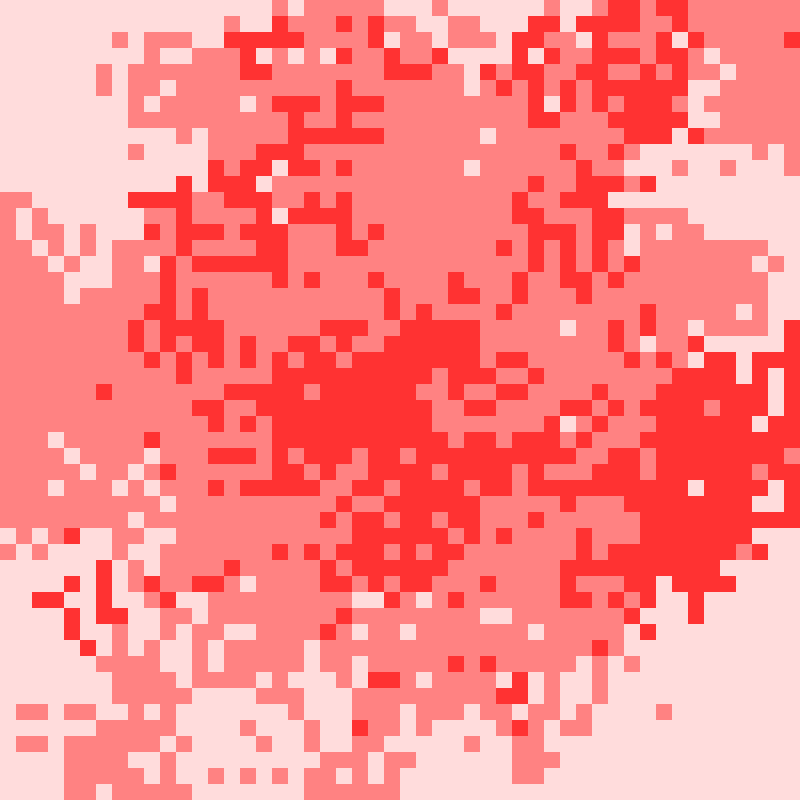
\includegraphics[width=.3\linewidth]{images/ca_25.png}
  }

  \subcaptionbox{$t = 50$}[.3\linewidth][c]{
    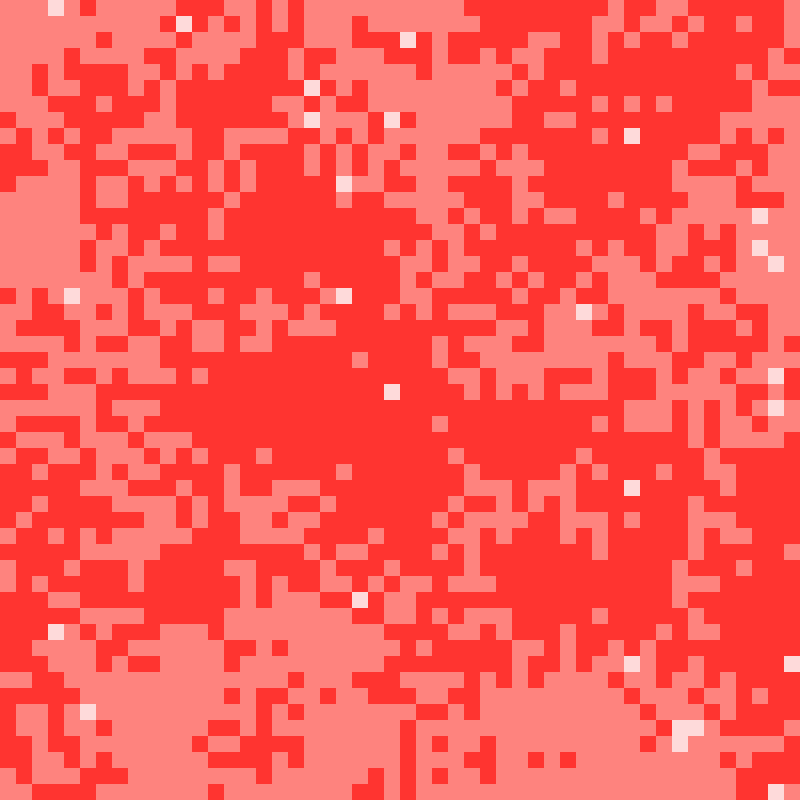
\includegraphics[width=.3\linewidth]{images/ca_50.png}
  }
  \subcaptionbox{$t = 100$}[.3\linewidth][c]{
    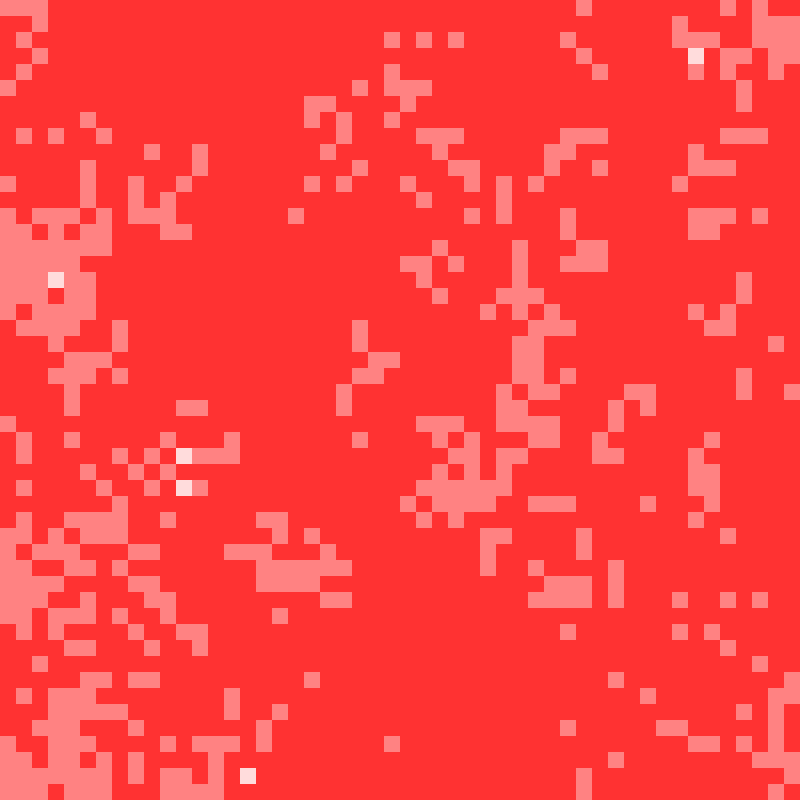
\includegraphics[width=.3\linewidth]{images/ca_100.png}
  }
  \caption{Quatre configurations de l'automate cellulaire. On y
    retrouve peu de similarités et les variations d'état sont trop
    rapides.}
  \label{fig:ac}
\end{figure}

\begin{figure}[H]
  \centering
  \subcaptionbox{}[.3\linewidth][c]{
    \raisebox{3cm}{$f(x) = \frac{1}{ 1 + e^{-x}}$}
  }
  \subcaptionbox{}[.6\linewidth][c]{
    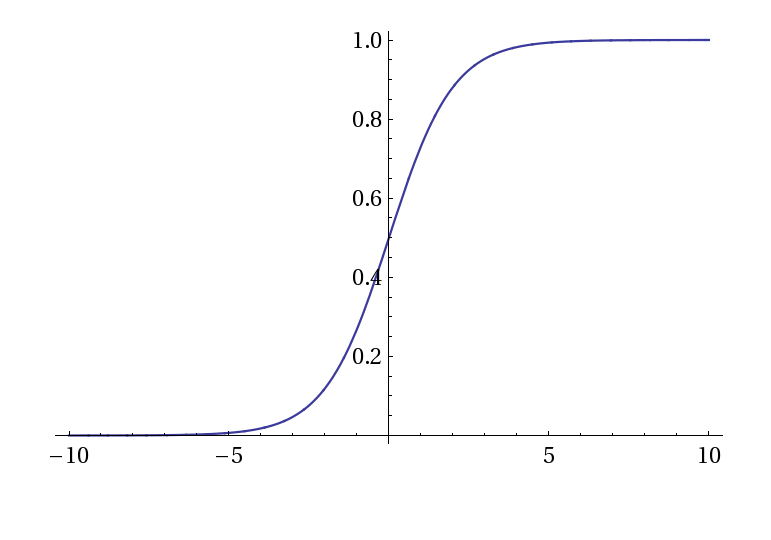
\includegraphics[width=.6\linewidth]{images/sigmoid.png}
  }
  \caption{Sigmoïde classique.}
  \label{fig:sigmoide1}
\end{figure}

\begin{figure}[H]
  \centering
  \subcaptionbox{}[.3\linewidth][c]{
    \raisebox{3cm}{$f(t) = \frac{1}{1 + e^{-0.02(t-350)}}$}
  }
  \subcaptionbox{}[.6\linewidth][c]{
    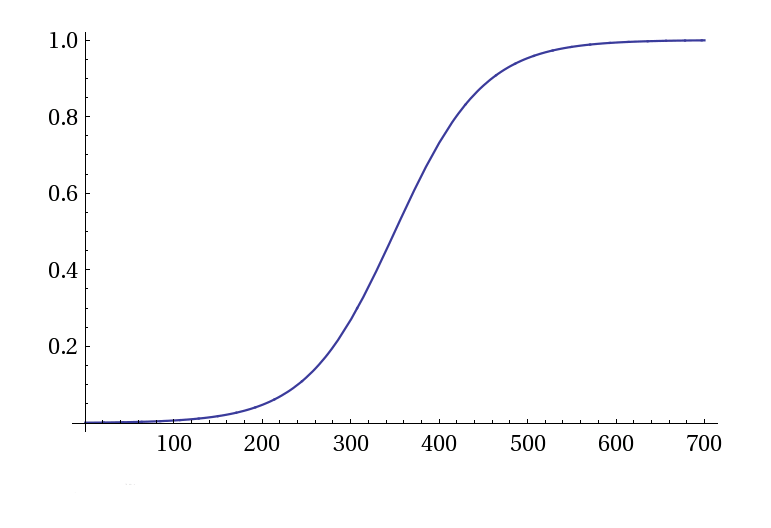
\includegraphics[width=.6\linewidth]{images/sigmoid-age.png}
  }
  \caption{Probabilité de changement d'état en fonction du temps.}
  \label{fig:sigmoide2}
\end{figure}

On voit sur la figure \ref{fig:ac-stable} un automate cellulaire doté
des mêmes règles de transition et de la même configuration initiale
que lors de notre première tentative mais pour lequel l'âge des
cellules est pris en compte lors de l'évaluation de la probabilité de
transition vers un autre état. En conséquence, l'évolution de la ville
est clairement ralentie et les modifications d'état locales ont le
temps de s'exprimer.

\begin{figure}[H]
  \centering
  \subcaptionbox{$t = 0$}[.3\linewidth][c]{
    
\includegraphics[width=.3\linewidth]{images/sca_0.png}
  }
  \subcaptionbox{$t = 500$}[.3\linewidth][c]{
    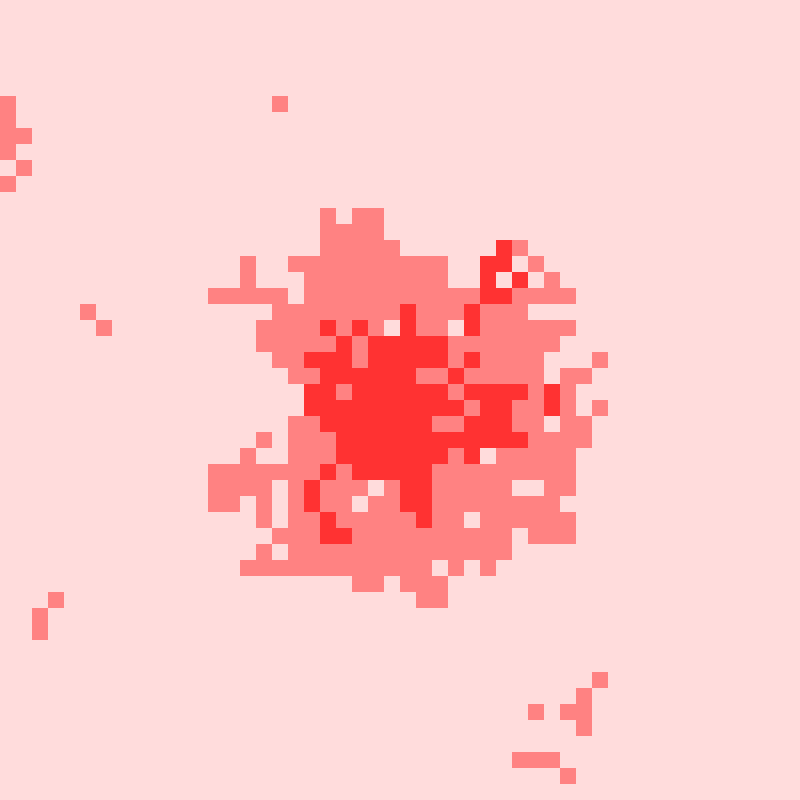
\includegraphics[width=.3\linewidth]{images/sca_500.png}
  }
  \subcaptionbox{$t = 1000$}[.3\linewidth][c]{
    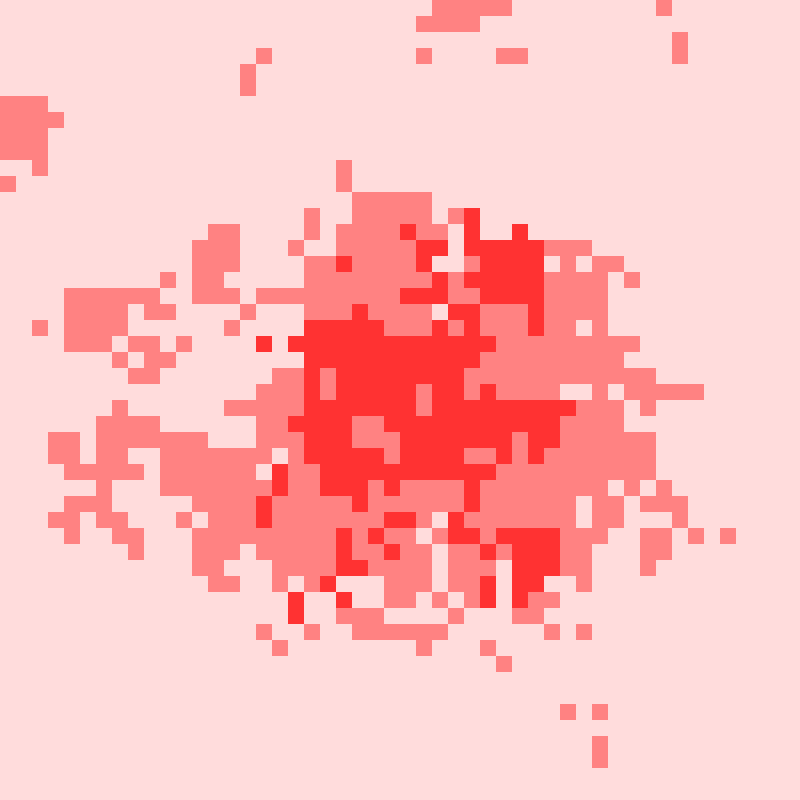
\includegraphics[width=.3\linewidth]{images/sca_1000.png}
  }

  \subcaptionbox{$t = 2000$}[.3\linewidth][c]{
    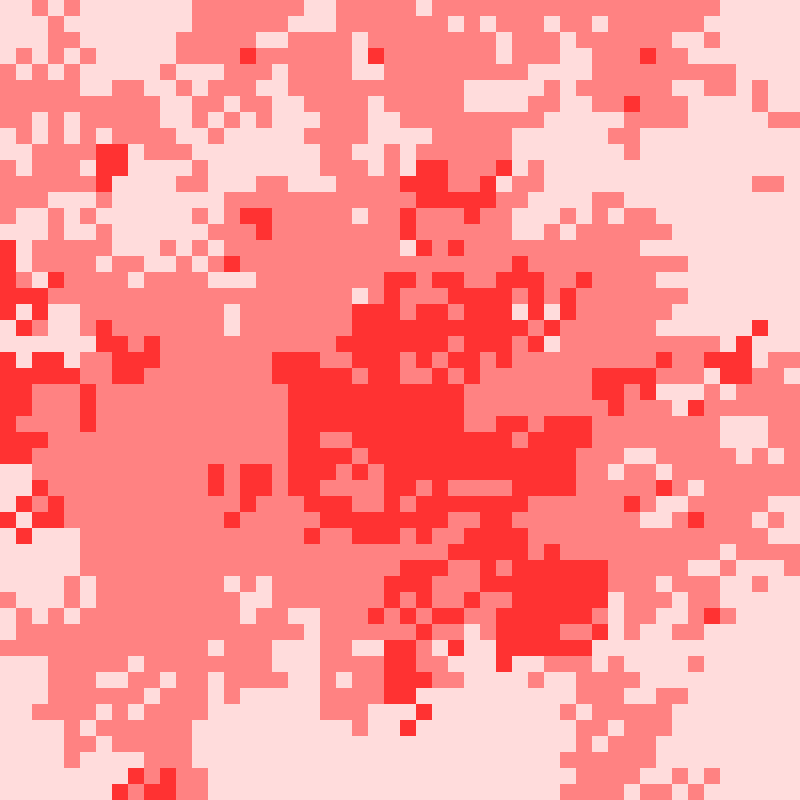
\includegraphics[width=.3\linewidth]{images/sca_2000.png}
  }
  \subcaptionbox{$t = 4000$}[.3\linewidth][c]{
    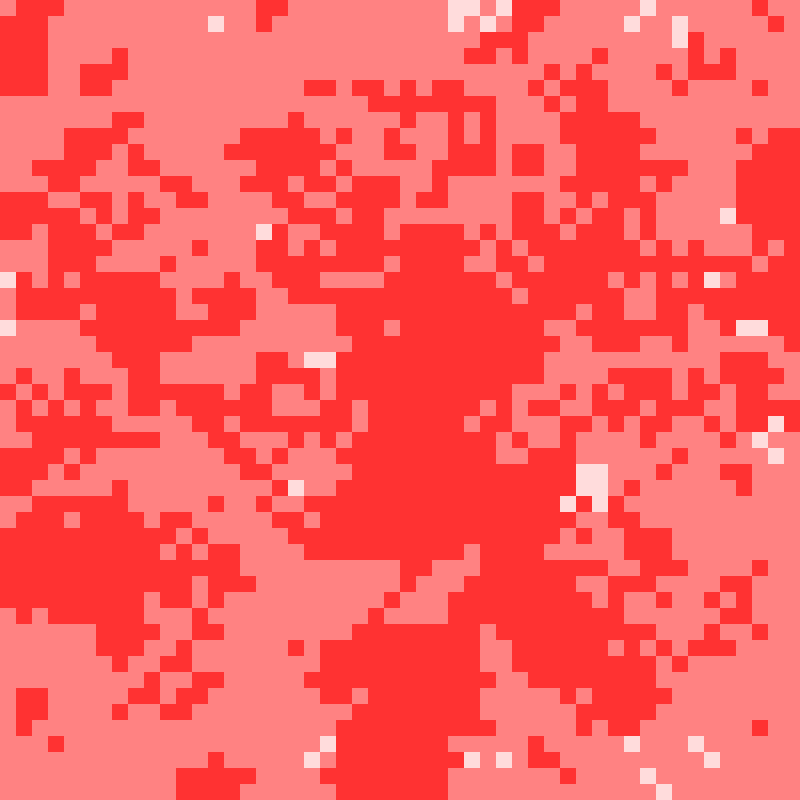
\includegraphics[width=.3\linewidth]{images/sca_4000.png}
  }
  \subcaptionbox{$t = 6000$}[.3\linewidth][c]{
    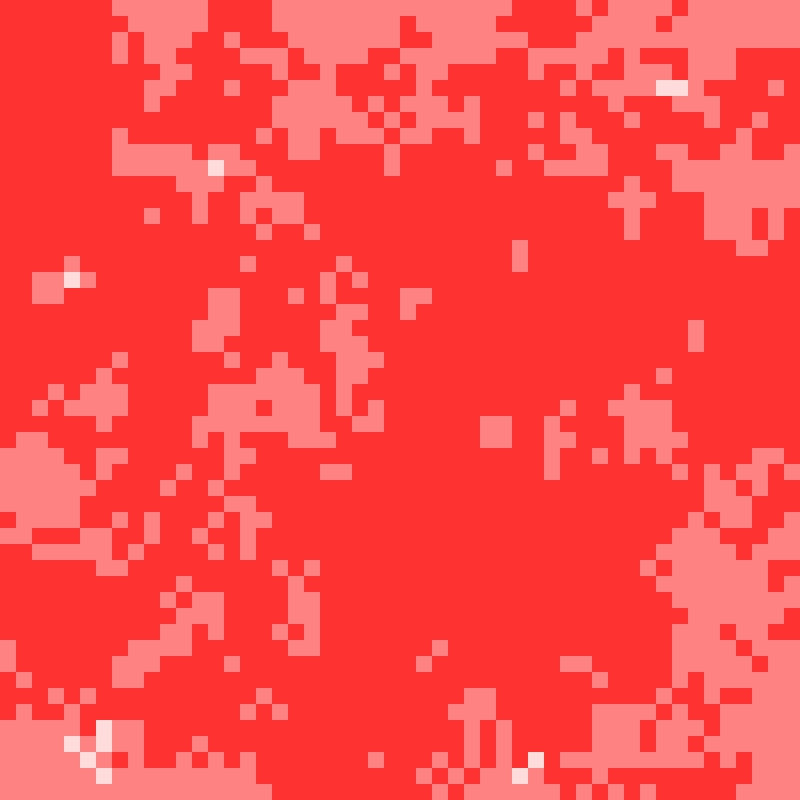
\includegraphics[width=.3\linewidth]{images/sca_6000.png}
  }
  \caption{Six configurations de l'automate cellulaire stabilisé.}
  \label{fig:ac-stable}
\end{figure}

Les exemples précédents permettent d'illustrer les règles de
transition et mettent en évidence un problème de stabilité et de
rythme à prendre en compte. Cependant, le but de cet exposé est de se
détacher de la régularité spatiale contraignante des automates
cellulaires et c'est à cet effet que l'on a présenté plus tôt le
diagramme de Voronoï. \`A la manière des automates cellulaires graphes
de O'Sullivan \cite{O'Sullivan2000}, chaque cellule de Voronoï voit
son état varier en fonction de son voisinage; voisinage établit à
partir de la topologie du diagramme; lui-même issu des positions des
centres des parcelles. On applique le même mécanisme cellulaire au
diagramme. La configuration initiale contient autant de parcelles que
l'automate cellulaire classique mais leur positionnement est aléatoire
(bien que que homogène). La progresion de l'évolution des densités est
visible sur la figure \ref{fig:ac-voronoi} et dévoile un comportement
similaire à celui observé sur l'automate cellulaire classique.

\begin{figure}[H]
  \centering
  \subcaptionbox{$t = 0$}[.3\linewidth][c]{
    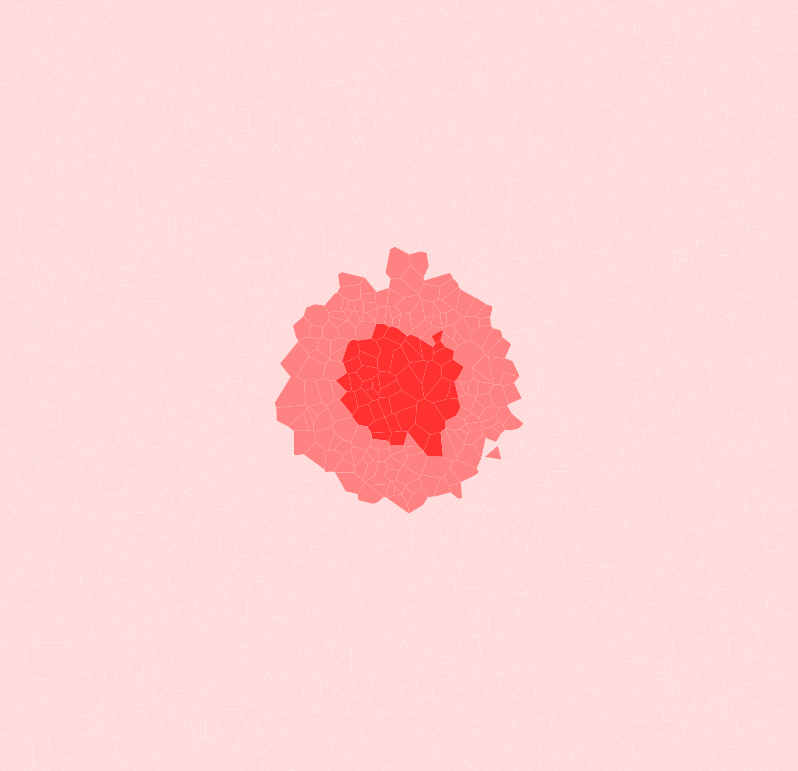
\includegraphics[width=.3\linewidth]{images/vca_0.png}
  }
  \subcaptionbox{$t = 500$}[.3\linewidth][c]{
    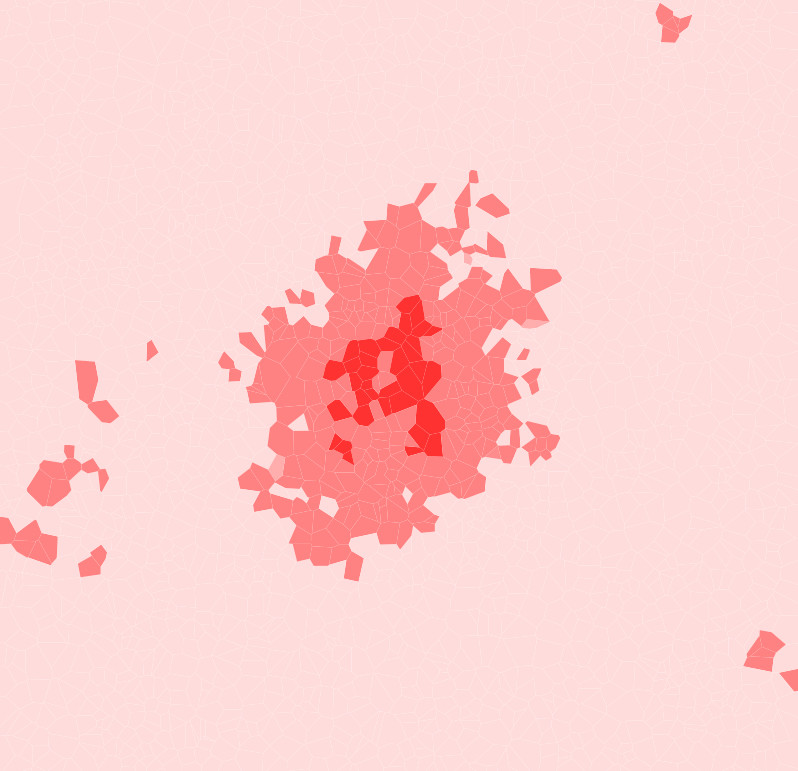
\includegraphics[width=.3\linewidth]{images/vca_500.png}
  }
  \subcaptionbox{$t = 1000$}[.3\linewidth][c]{
    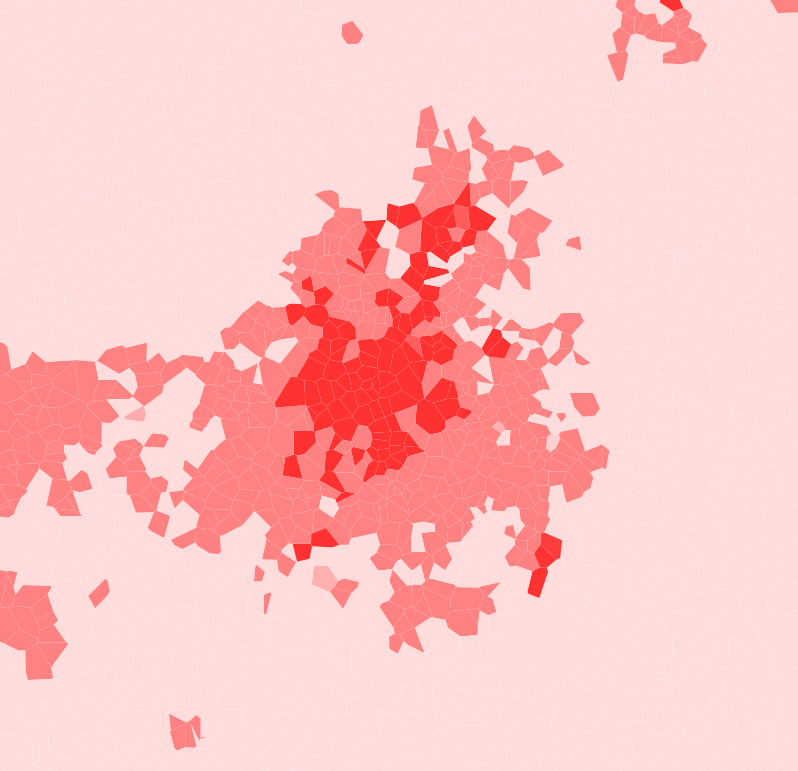
\includegraphics[width=.3\linewidth]{images/vca_1000.png}
  }

  \subcaptionbox{$t = 2000$}[.3\linewidth][c]{
    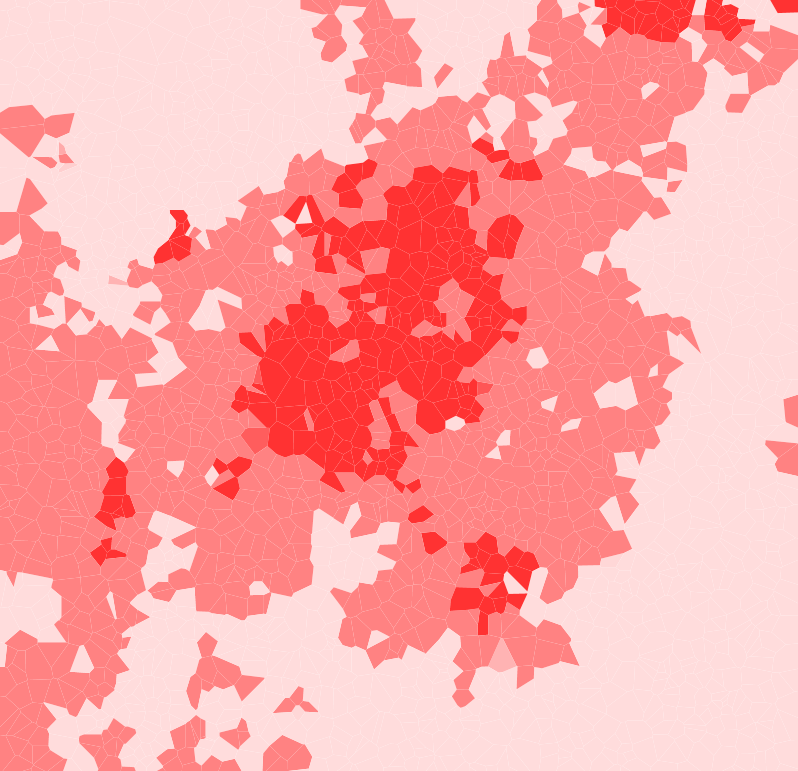
\includegraphics[width=.3\linewidth]{images/vca_2000.png}
  }
  \subcaptionbox{$t = 4000$}[.3\linewidth][c]{
    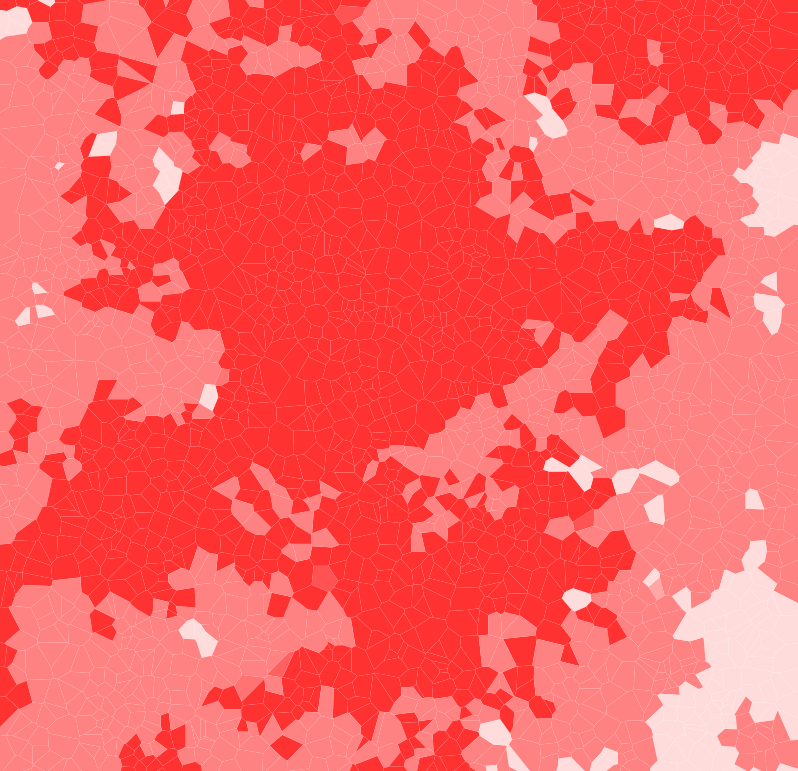
\includegraphics[width=.3\linewidth]{images/vca_4000.png}
  }
  \subcaptionbox{$t = 6000$}[.3\linewidth][c]{
    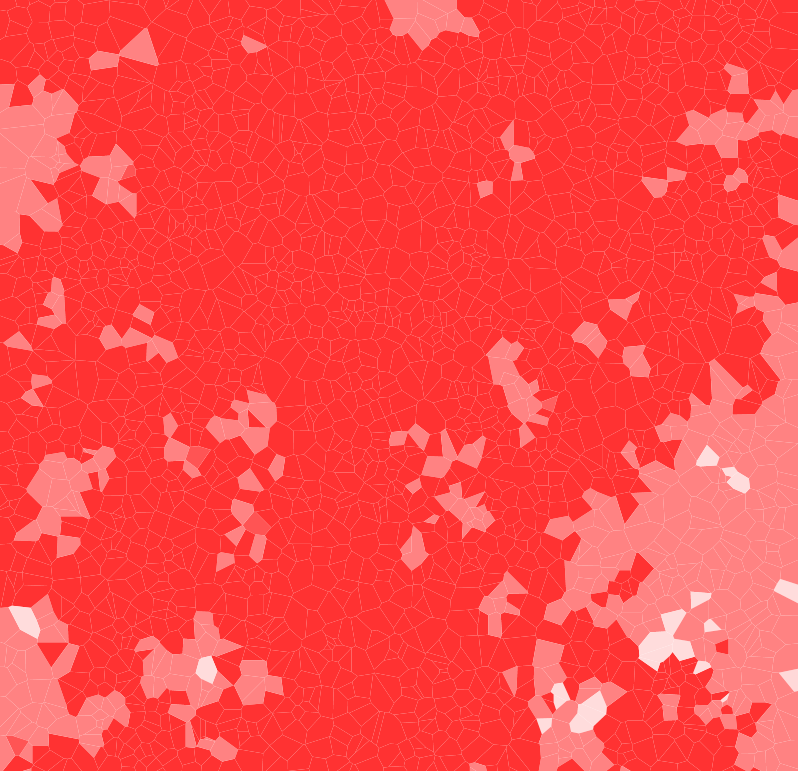
\includegraphics[width=.3\linewidth]{images/vca_6000.png}
  }
  \caption{Six configurations du diagramme de Voronoï cellulaire.}
  \label{fig:ac-voronoi}
\end{figure}

Plus la simulation avance et plus le système est chargé de parcelles à
haute densité. Un lecteur averti pourrait argumenter que ce
comportement est bien différent de ce que l'on peut constater en
situation réelle : quel que soit le taux de croissance d'une ville,
elle ne finit jamais entièrement remplie de grands immeubles et de
centres commerciaux. Mais il faut garder à l'esprit que le mécanisme
présenté dans cette section ne gère que la croissance verticale. Par
la suite, la croissance horizontale de la ville étendra ses frontières
de façon à ce que les nouvelles parcelles à sa bordure soient moins
denses.

La problématique étant d'étudier la coévolution de deux aspects
urbains, le viaire et le bâti, et non seulement l'évolution des
densités (qui ne sert que de support à l'essort de la ville), on a
préféré choisir une règle basique. Il est néanmoins tout à fait
possible d'utiliser par la suite des règles cellulaires plus
sophistiquées pour améliorer le réalisme de la simulation. On
pourrait, par exemple, prendre en compte les valeurs financières des
parcelles ou les classes sociales des habitants.

\subsubsection{Placement des éléments potentiels}

Le second mécanisme place de nouveaux éléments urbains en bordure de
la ville et est ainsi responsable de sa croissance horizontale. Ces
éléments sont les routes et les parcelles mais il est seulement
nécessaire de considérer le placement de ces dernières. En effet, les
voies sont représentées par les arêtes de la cellule de Voronoï
associé à une parcelle.

En quelques mots, le placement se déroule comme suit :

\begin{enumerate}
\item{On détermine les centres de la ville en fonction de la densité}
\item{On dépose sur un des centres une \textit{graine} mobile qui
  servira de générateur à la nouvelle parcelle;}
\item{La graine se déplace sous l'influence des variables immanentes à
  la ville;}
\item{Quand la graine stoppe son mouvement, on y crée la parcelle.}
\end{enumerate}

Le déplacement de la graine est un processus pouvant potentiellement
prendre en compte de nombreuses variables. Dans la simulation
d'exemple que l'on décrit, seules la densité et le placement des
routes peuvent guider la graine, car ce sont les uniques données
considérées. Cependant, on souhaite que le modèle soit extensible et
qu'il soit capable de supporter d'autres variables et contraintes : la
valeur des sols par exemple, ou bien la pente des zones envisagées ou
l'impossibilité de s'installer sur certains types de terrain (forêts,
plans d'eau). De cette idée de graine se déplaçant en fonction
d'influences diverses transpire un véritable aspect physique.

On emploie donc une approche mécanique qui se base sur un champ de
vecteurs généré à partir de l'état du sytème urbain pour guider la
graine vers sa destination. Puisque de nombreux paramètres sont à
prendre en compte, on utilise un champ de vecteurs par donnée que l'on
souhaite exprimer puis on les combine; ce qui permet de pondérer
différemment l'impact de chaque donnée.

On veut évidemment que la densité soit prise en compte dans ce
placement. Dans une ville, les nouvelles installations ont
principalement tendance à se répartir sur les frontières de
l'enveloppe urbaine et à s'éloigner des centres, non pas par animosité
envers l'activité du centre-ville mais simplement par manque
d'espace. Pour traduire ce phénomène dans le modèle, un premier champ
$I_d$ fait donc pointer chacun de ses vecteurs vers la parcelle
disposant de la plus faible densité parmis les voisines de la parcelle
sur laquelle il est posé. Ainsi des chemins de vecteurs se forment et
mènent vers les zones à densité réduite.

Il est aussi naturel que les nouvelles parcelles soient placées près
des installations routières existantes de façon à pouvoir communiquer
aisément avec les grands axes routiers. À cet effet, on ajoute un
champ $I_r$ pour lequel chaque vecteur pointe vers la voie construite
la plus proche. Dans notre modèle, les voies ne sont pas hiérarchisées
et on ne fait de distinction entre les routes primaires, secondaires
et tertiaires. Si c'était le cas, on pourrait cependant imaginer
adjoindre à chaque route des coefficients différents selon leur classe
afin que les grands axes attirent le bâti et que les ruelles aient un
impact moindre.

Les nouvelles parcelles ne sont pas uniquement disposés en fonction de
variables internes à la ville car, souvent, l'environnement impose des
restrictions quant à la direction que son expansion va prendre. Parmi
ces contraintes, on pense aux zones non constructibles comme les plans
d'eau, les forêts mais aussi aux fortes pentes. Un champ de vecteurs
$I_o$ est dédié à l'évitement de telles zones et repousse la graine
des obstacles.

L'influence générale qu'a le champ de vecteurs final $I$, somme
pondérée de tous les autres, à la position $(x,y)$ est donnée par
l'équation \ref{eq:vf}. Les facteurs $\alpha$, $\beta$ et $\gamma$
sont à définir en fonction de l'importance que l'on souhaite donner à
chaque champ et donc à l'information qu'ils expriment.

\begin{equation}
  I(x,y) = \alpha I_d(x,y) + \beta I_r(x,y) + \gamma I_o(x,y)
  \label{eq:vf}
\end{equation}

Pour calculer $I_k(x,y)$ avec $k \in \{d,r,o\}$, on identifie les
quatres vecteurs entourant le point $(x,y)$ puis on effectue une
interpolation bilinéaire pour obtenir la valeur qu'aurait un vecteur
en $(x,y)$.

Afin d'illustrer ce mécanisme, une ville virtuelle et les champs de
vecteurs associés sont visibles sur la figure \ref{fig:fields}. Plus
les parcelles arborent une couleur vive et plus leur densité est
élevée. Le quart de cercle gris correspond à un obstacle. Les arêtes
bleues forment un axe viaire. La combinaison des trois champs de
vecteurs fournit le champs final de la figure \ref{fig:field-sum}. Les
chemins qui s'y forment guident vers les bords ouest et est de la
ville par attirance de l'axe routier mais aussi dans une moindre
mesure vers le nord et le sud. La croissance vers le sud-est est
stoppé par l'influence de l'obstacle.

On remarque que cette ville ne contient qu'une unique route passant
horizontalement par son centre. En conséquence, la majeure partie des
parcelles n'est pas reliée au réseau routier. Cette configuration
jouet n'est donc aucunement réaliste mais permet d'illustrer la
formation des champs de vecteurs.

\begin{figure}[H]
  \centering \subcaptionbox{Ville virtuelle.}[.45\linewidth][c]{
    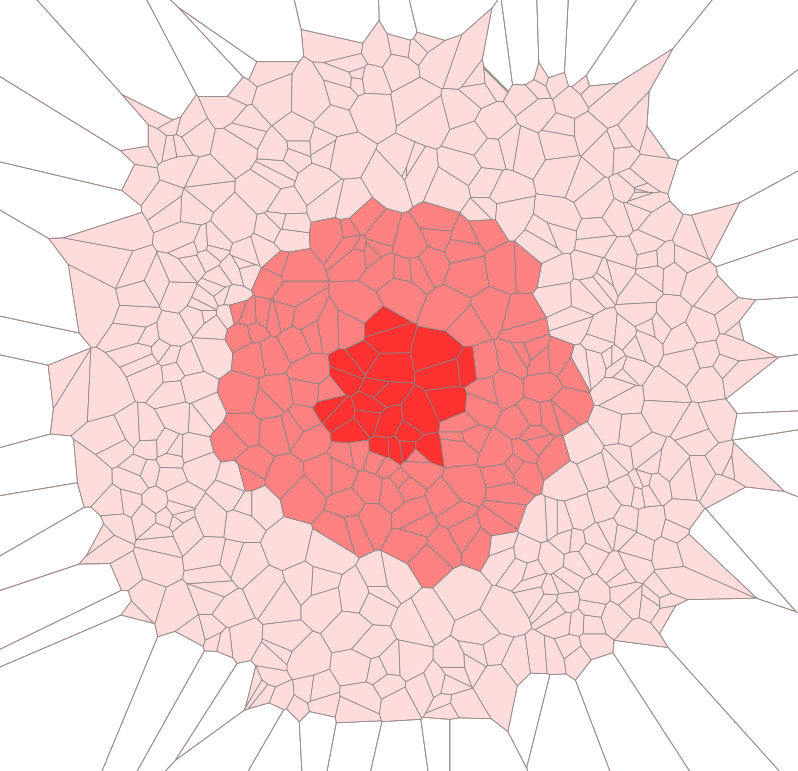
\includegraphics[width=.45\linewidth]{images/vf-base.png}
  }
  \subcaptionbox{$I_d$, le champ d'évasion de la
    densité.}[.45\linewidth][c]{
    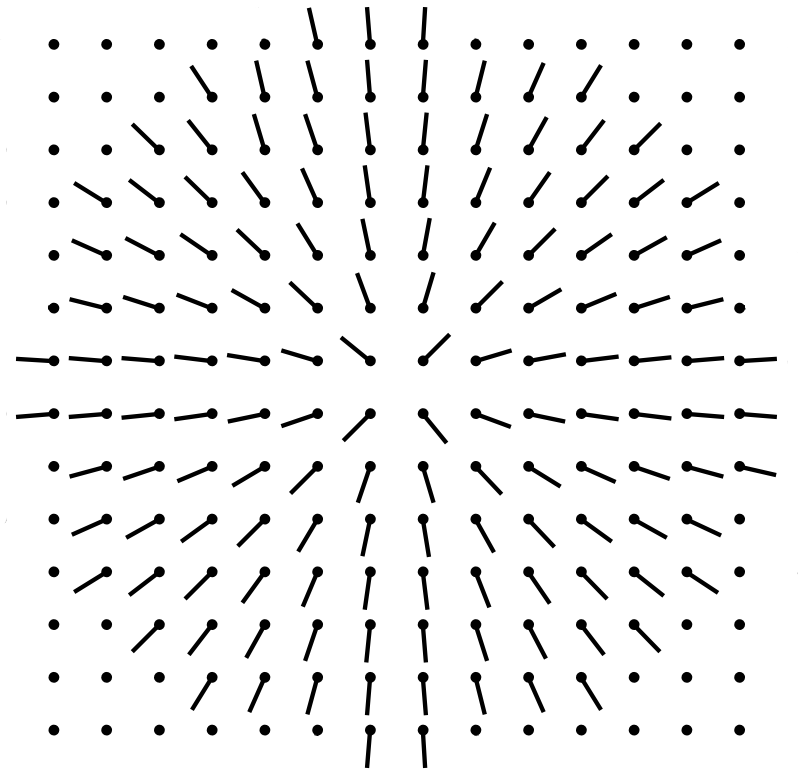
\includegraphics[width=.45\linewidth]{images/vf-density.png}
  }

  \subcaptionbox{$I_r$, Le champ d'attraction des routes}[.45\linewidth][c]{
    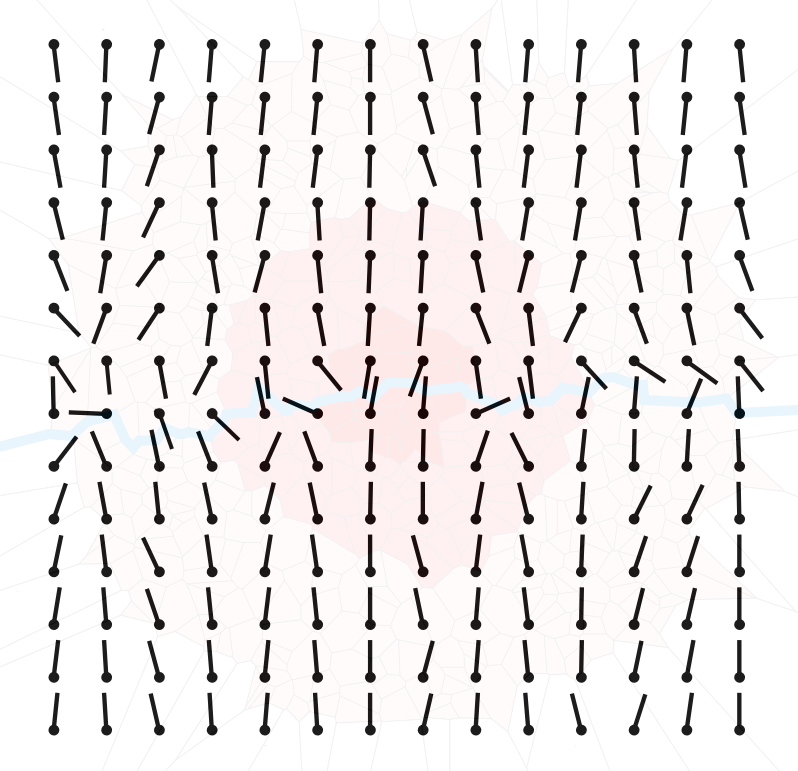
\includegraphics[width=.45\linewidth]{images/vf-road.png}
  }
  \subcaptionbox{$I_o$, le champ de répulsion des obstacles}[.45\linewidth][c]{
    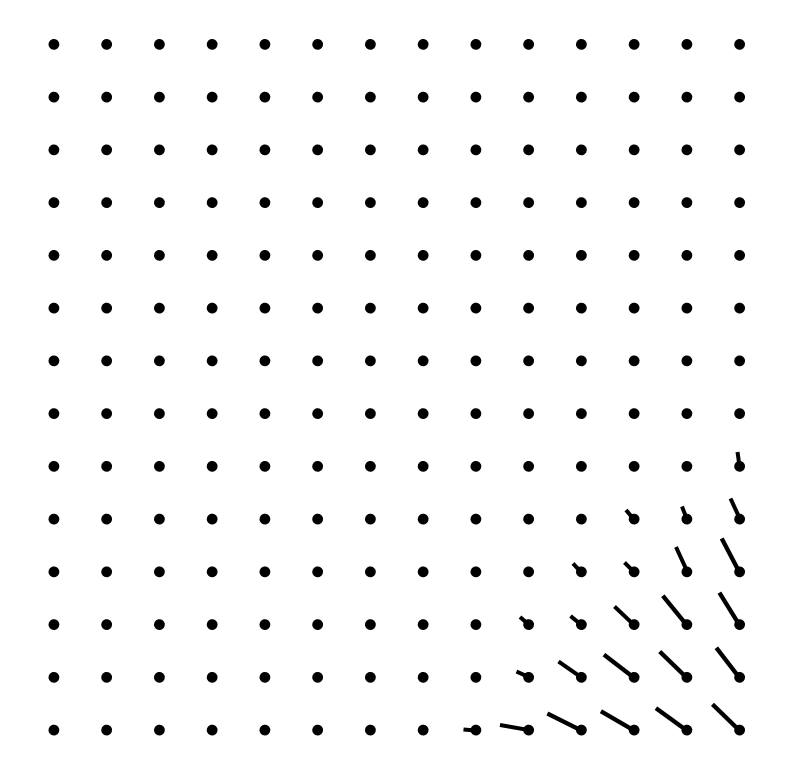
\includegraphics[width=.45\linewidth]{images/vf-obstacle.png}
  }
  \caption{Une ville virtuelle et les différentes influences y guidant
    le positionnement des nouvelles parcelles.}
  \label{fig:fields}
\end{figure}

\begin{figure}[H]
  \centering
  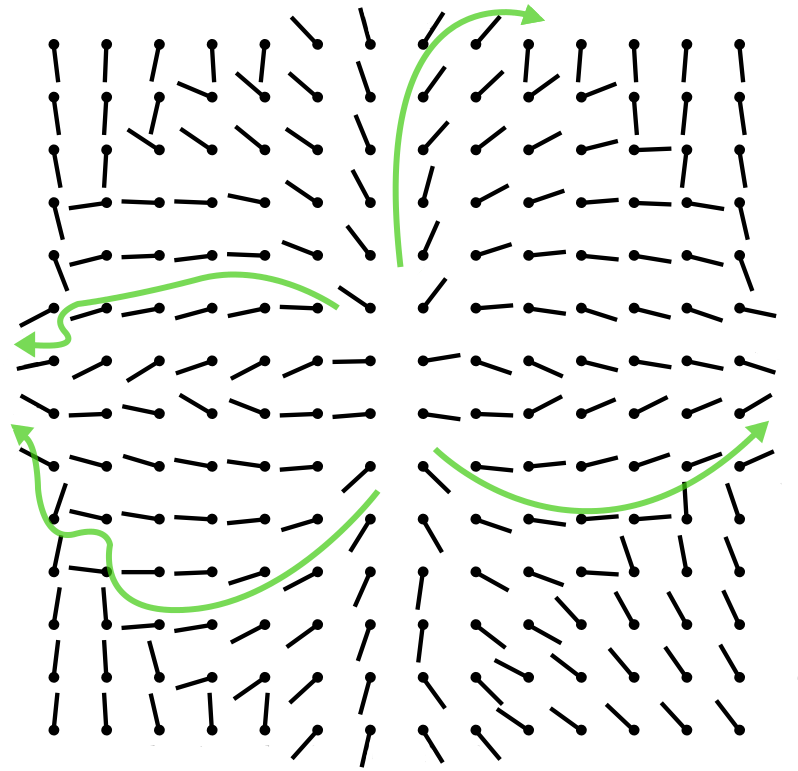
\includegraphics[width=.8\linewidth]{images/vf-sum.png}
  \caption{}
  \label{fig:field-sum}
\end{figure}

VITESSE DE LA GRAINE

ARRET DE LA GRAINE

TRACER CHEMIN GRAINE

Les quelques champs de vecteurs décrit ci-dessus servent un but
illustratif. La généralité de ce mécanisme permet à l'utilisateur du
modèle d'employer les données qu'il juge nécessaires afin de mettre en
avant certaines caractéristiques d'un système urbain. Utiliser ces
trois champs permet de guider la croissance de la ville en fonction
des quantités qui la représentent et de contraintes de
l'environnement. Il serait aussi utile de bénéficier de moyens de
contrôle sur cette évolution urbaine. Dans les villes, des motifs
réguliers se dessinent et sont issus d'un besoin d'organisation de
l'espace. On pense notamment à l'organisation en grille typique de
Manhattan ou à l'organisation radiale de certains quartiers. Afin
d'imposer ce type de placement, il serait envisageable d'employer un
nouveau champ de vecteurs guidant vers des points fixes. TOujours dans
une optique de contrôle, on peut utiliser un champ guidant les
nouvelles parcelles vers des zones d'attraction dont une municipalité
souhaiterait évaluer le potentiel.

\subsubsection{Construction des éléments potentiels}

Le mécanisme de placement des élément potentiels présenté précédemment
se base sur les variables internes au système urbain; variables dont
l'évolution est régie par le mécanisme cellulaire. Seulement, les
nouvelles parcelles et routes placées sont potentielles. Le troisième
mécanisme choisit parmi ces éléments potentiels lesquels sont
construits. On traite différemment le choix des parcelles à construire
et le choix des routes à construire.

\paragraph{Choix des parcelles\\}

Afin de contrôler l'expansion effective de la ville, un taux de
croissance $c_p$ est défini pour régler la vitesse de construction des
parcelles potentielles. $c_p$ parcelles sont construites par itération
du modèle.

Toujours dans un soucis de cohérence historique, on refuse qu'une
parcelle potentielle soit construite alors qu'elle n'est pas encore
reliée au réseau routier existant. On considère donc uniquement celles
dont la cellule de Voronoï a au moins une arête construite.

Une fois ces parcelles candidates listées, on leur adjoint un score
fonction de l'âge de leur prévision (le temps auquel elles ont été
placées). Le but de cette quantification est de donner la priorité de
construction aux parcelles prévues depuis plus longtemps. La ville
étant néanmoins une structure imparfaite et parfois désordonnée, le
choix des parcelles est fait par un tirage aléatoire biaisé en
fonction de ce score et la priorité par l'âge n'est pas garantie.

ETOFFER

\paragraph{Choix des routes\\}

La construction des routes potentielles est un problème plus
complexe. Le diagramme de Voronoï, et plus précisément ses arêtes et
sommets, forment un réseau routier global dans lequel chaque parcelle
est encerclée de routes potentielles. Dans une ville réelle, toutes
les parcelles ne sont bien sûr pas entourées de voies mais sont
regroupées en blocs ou en bandes elles-mêmes encerclées. La tâche à
accomplir est donc de sélectionner des arêtes du réseau routier global
pour les construire.

REFORMULER

NETWORK SIMPLEX

UN PUIT + PLUSIEURS SOURCES

EVALUATION

\section{Mesures}

\subsection{Démonstration}

Afin d'évaluer notre modèle, on l'applique à une configuration
réelle. La zone géographique étudiée est la partie ouest du Havre. Les
données utilisées \footnote{Les données employées proviennent de
  l'Agence Européenne pour l'Environnement
  \url{http://www.eea.europa.eu/data-and-maps/data/urban-atlas}} ont
été réduites à un sous-espace de la ville pour des raisons de temps de
calcul. Elles comprennent les informations cadastrales, les densités
de population et le tracé du réseau routier.

AJUSTER IMAGES

\begin{figure}[H]
  \centering
  \subcaptionbox{Vue aérienne.}[.3\linewidth][c]{
    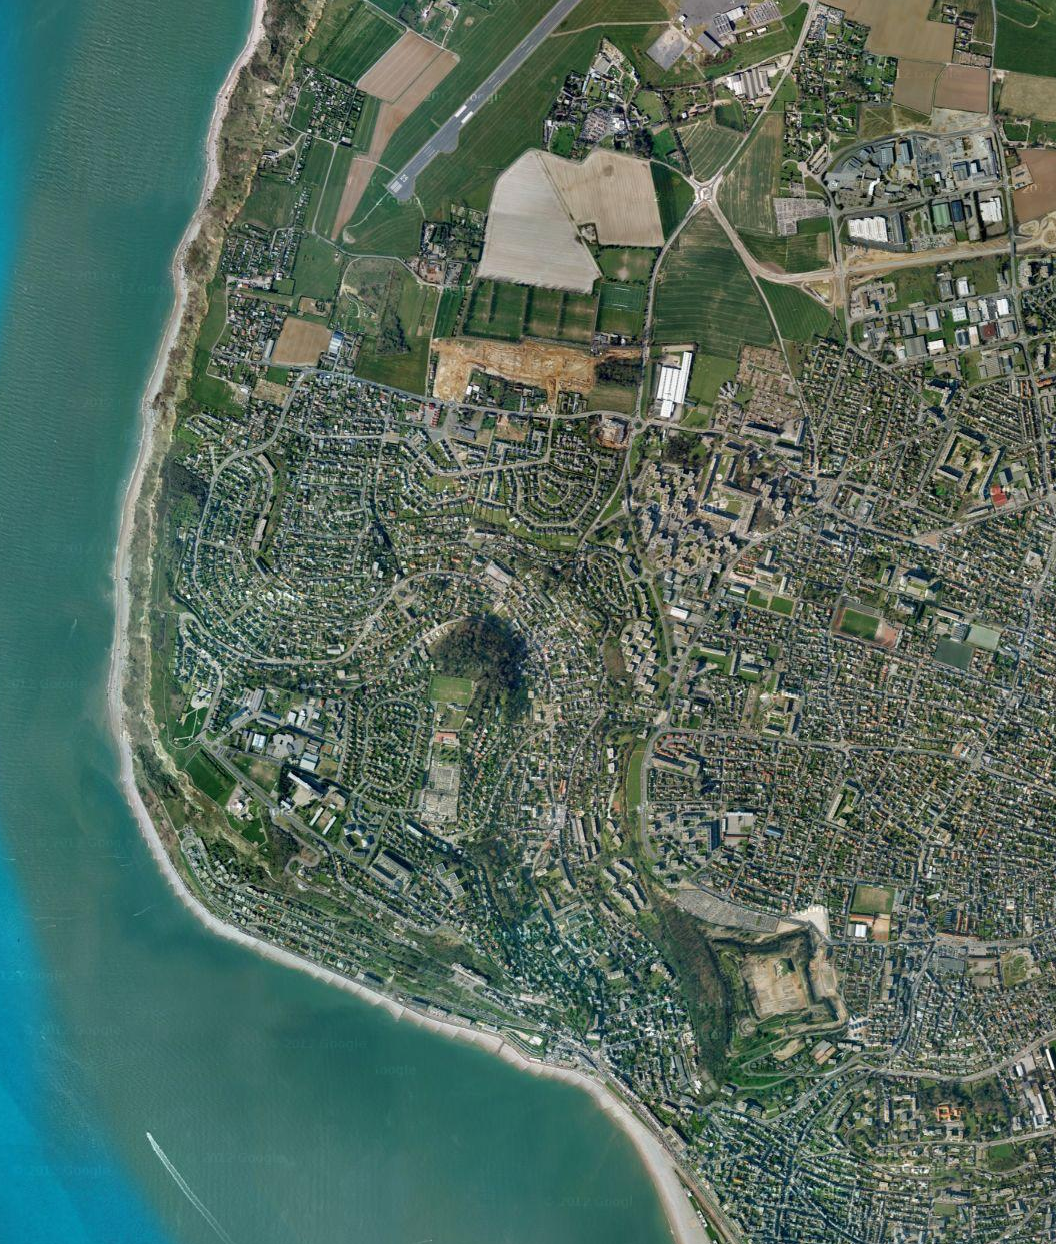
\includegraphics[width=.3\linewidth]{images/le_havre_map.png}
  }
  \subcaptionbox{Shapefile.}[.3\linewidth][c]{
    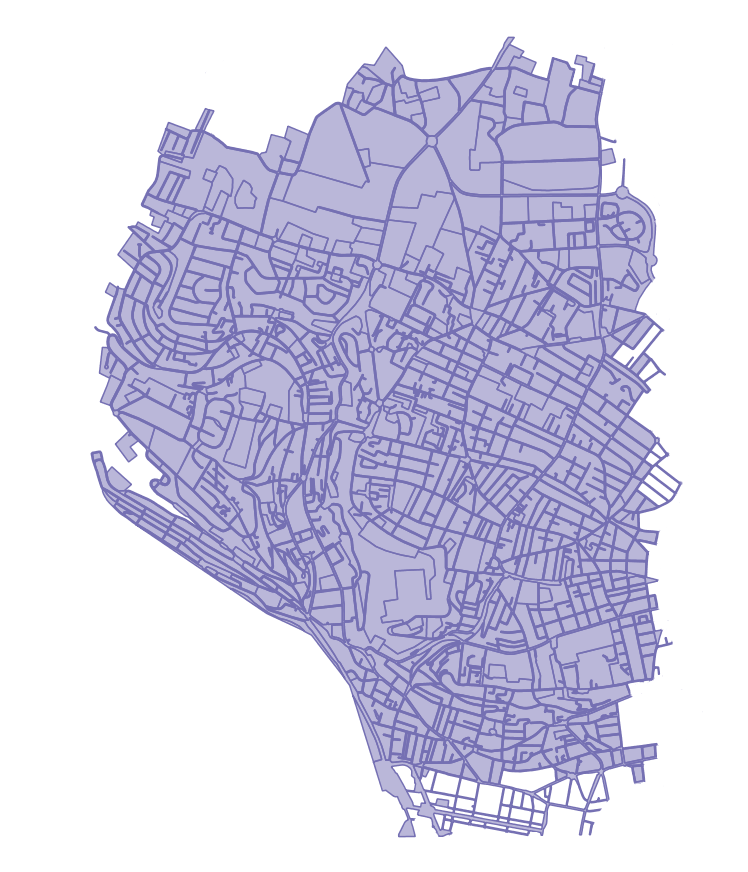
\includegraphics[width=.3\linewidth]{images/le_havre_shapefile.png}
  }
  \subcaptionbox{Diagramme de Voronoï.}[.3\linewidth][c]{
    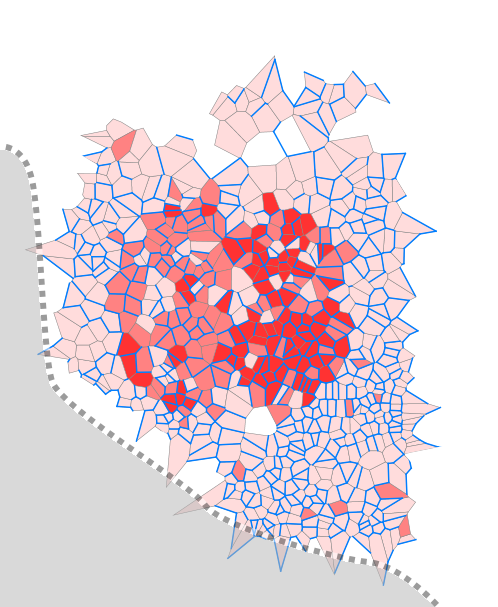
\includegraphics[width=.3\linewidth]{images/le_havre_voronoi.png}
  }
  \caption{}
  \label{fig:le_havre}
\end{figure}

PROFIL COTIER = OBSTACLE

\begin{figure}[H]
  \centering
  \subcaptionbox{$t = 0$}[.45\linewidth][c]{
    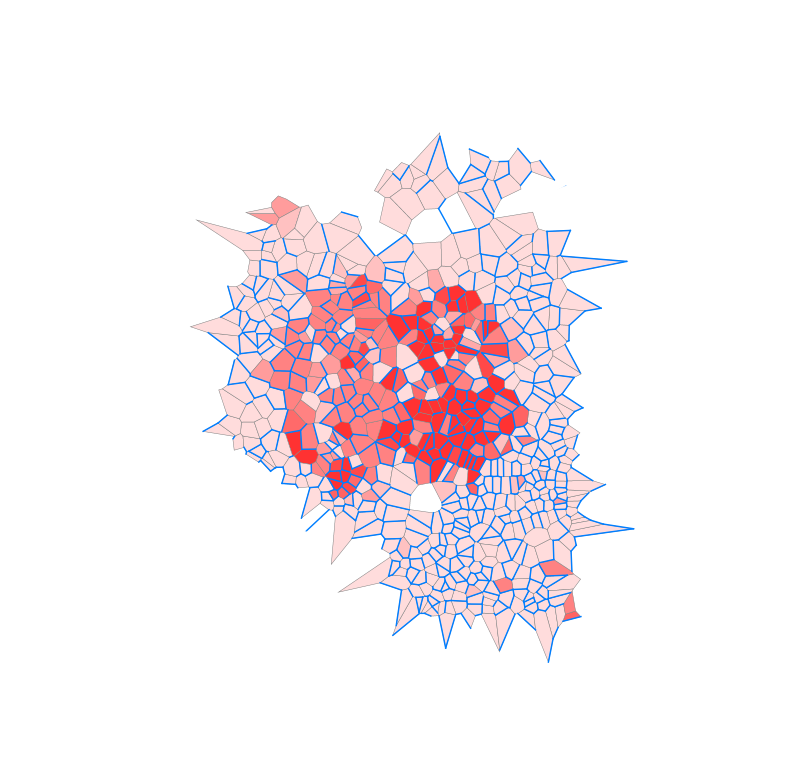
\includegraphics[width=.45\linewidth]{images/lh_0.png}
  }
  \subcaptionbox{$t = 100$}[.45\linewidth][c]{
    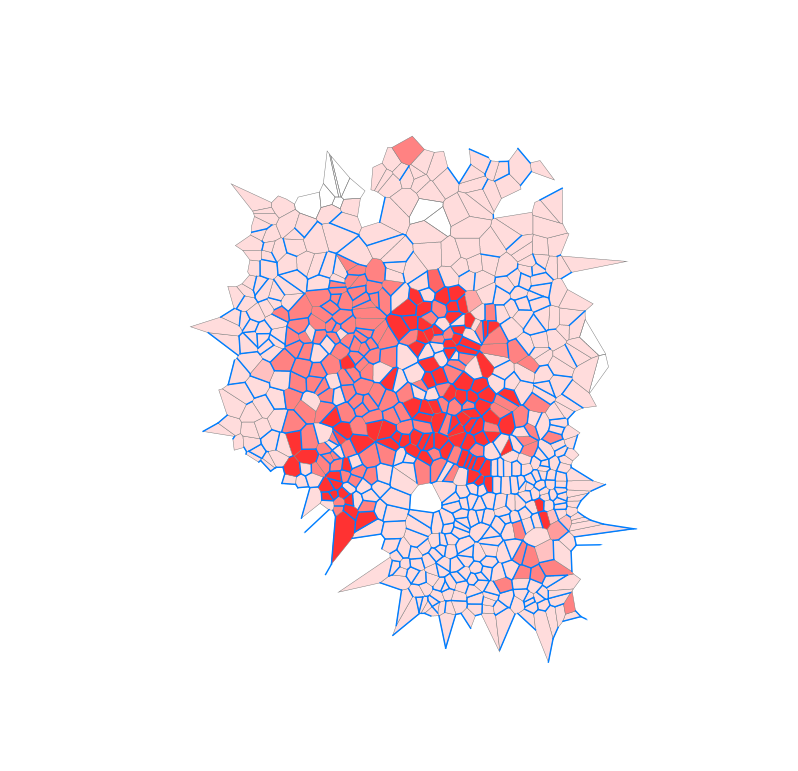
\includegraphics[width=.45\linewidth]{images/lh_100.png}
  }

  \subcaptionbox{$t = 200$}[.45\linewidth][c]{
    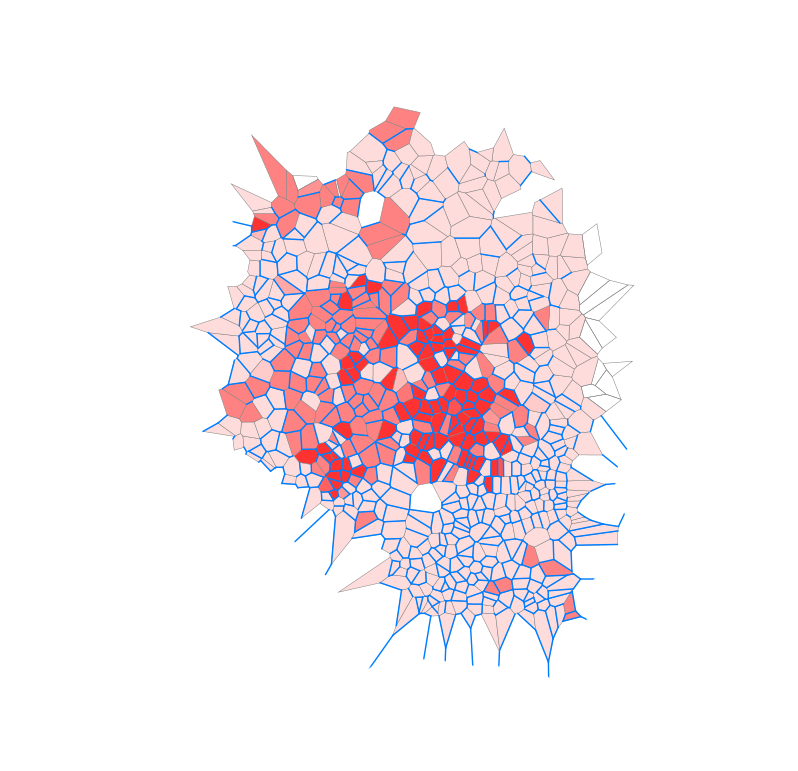
\includegraphics[width=.45\linewidth]{images/lh_200.png}
  }
  \subcaptionbox{$t = 300$}[.45\linewidth][c]{
    \includegraphics[width=.45\linewidth]{images/lh_300.png}
  }

  \subcaptionbox{$t = 400$}[.45\linewidth][c]{
    \includegraphics[width=.45\linewidth]{images/lh_400.png}
  }
  \subcaptionbox{$t = 500$}[.45\linewidth][c]{
    \includegraphics[width=.45\linewidth]{images/lh_500.png}
  }
  \caption{Évolution de notre Havre partiel sur 500 itérations.}
  \label{fig:le_havre_demo}
\end{figure}

IMAGE COMPARAISON T0 T500

NOUVEAUX CENTRES

CROISSANCE NORD ET EST

\subsection{Mesures sur le bâti}

\subsubsection{Évolution de la superficie de la ville}

\begin{figure}[H]
  \centering
  \includegraphics[width=.8\linewidth]{images/area.png}
  \caption{}
\end{figure}

LINEAIRE

DEVRAIT SE STABILISER

\subsubsection{Évolution de la superficie par densité}

\begin{figure}[H]
  \centering
  \includegraphics[width=.8\linewidth]{images/area_ALL.png}
  \caption{}
\end{figure}

\subsection{Mesures sur le viaire}

\subsubsection{Diamètre}

A FAIRE

\begin{figure}[H]
  \centering
  %\includegraphics[width=.8\linewidth]{images/area.png}
  \caption{}
\end{figure}

\subsubsection{Centralité}

A FAIRE

\begin{figure}[H]
  \centering
  %\includegraphics[width=.8\linewidth]{images/area.png}
  \caption{}
\end{figure}

\subsubsection{Degré des carrefours}

\begin{figure}[H]
  \centering
  \includegraphics[width=.8\linewidth]{images/degree.png}
  \caption{}
\end{figure}

COMMENCE BAS -> APPROXIMATION

STABILISE

CARACTERISTIQUE

\subsubsection{Degré des carrefours selon la distance}

\begin{figure}[H]
  \centering
  \includegraphics[width=.8\linewidth]{images/degree_distance.png}
  \caption{}
\end{figure}



\section{Conclusion}

RESUME

CONSTAT

PERSPECTIVES

\printbibliography

\end{document}
